\chapter{เมทริกซ์และดีเทอร์มิแนนต์ (Matrices \& Determinants)}
\label{ch:matrix}
\label{sec:matrix-intro}

เมทริกซ์ (Matrix) เป็นโครงสร้างข้อมูลทางคณิตศาสตร์ที่ใช้จัดระเบียบข้อมูลในรูปแบบตารางสองมิติ เมทริกซ์ประกอบด้วยแถว (rows) และคอลัมน์ (columns) โดยแต่ละช่องเก็บค่าที่เรียกว่าสมาชิก (element) หรือค่าประจำตำแหน่ง (entry) ของเมทริกซ์ การจัดระเบียบข้อมูลในรูปแบบนี้ทำให้สามารถดำเนินการทางคณิตศาสตร์ได้อย่างมีประสิทธิภาพและเป็นระบบ ในเชิงทฤษฎี เมทริกซ์สามารถมองได้ว่าเป็นการแทนเชิงเส้น (linear transformation) ระหว่างปริภูมิเวกเตอร์ ซึ่งเป็นหัวใจสำคัญของพีชคณิตเชิงเส้นที่วางรากฐานให้กับขั้นตอนวิธีทางคอมพิวเตอร์จำนวนมาก~\cite{anton2019linear, strang2023linear}

เมทริกซ์ถูกใช้อย่างกว้างขวางในวิทยาการคอมพิวเตอร์และคณิตศาสตร์ประยุกต์ เนื่องจากเป็นพื้นฐานของคอมพิวเตอร์กราฟิกส์ (การแปลงภาพ 2 มิติและ 3 มิติ) การเรียนรู้ของเครื่อง (Neural Networks) การเข้ารหัส (Hill Cipher) และการแก้ระบบสมการเชิงเส้น ในงานด้านการประมวลผลภาพ เมทริกซ์คอนโวลูชัน (Convolution Matrix) ถูกใช้ในการทำ blur, sharpen และ edge detection ขณะที่ในด้านการเรียนรู้ของเครื่อง เมทริกซ์น้ำหนัก (weight matrices) เป็นองค์ประกอบหลักของโครงข่ายประสาทเทียม นอกจากนี้เมทริกซ์ยังถูกใช้ในงานด้านการวิเคราะห์ข้อมูล การคำนวณทางวิทยาศาสตร์หลากหลายสาขา และการแก้ปัญหาเชิงการจัดการเครือข่ายผ่านเมทริกซ์ประชิด (Adjacency Matrix) ในทฤษฎีกราฟ

ประวัติศาสตร์ของเมทริกซ์เริ่มต้นในช่วงต้นศตวรรษที่ 19 โดย Arthur Cayley และ William Rowan Hamilton ซึ่งเป็นผู้ให้คำนิยามและพัฒนาทฤษฎีเมทริกซ์อย่างเป็นระบบ ถึงแม้ว่าแนวคิดเรื่องดีเทอร์มิแนนต์จะมีมาก่อนหน้านี้โดยนักคณิตศาสตร์ชาวญี่ปุ่นและยุโรป เช่น Seki Kowa ในศตวรรษที่ 17 และ Gottfried Leibniz ในศตวรรษที่ 18 ซึ่งต่างก็ใช้ดีเทอร์มิแนนต์ในการแก้ระบบสมการเชิงเส้น การพัฒนาทฤษฎีเมทริกซ์อย่างเป็นระบบได้วางรากฐานให้กับคณิตศาสตร์ขั้นสูงหลายสาขา รวมถึงพีชคณิตเชิงเส้น (Linear Algebra) ที่มีบทบาทสำคัญในการพัฒนาขั้นตอนวิธีทางคอมพิวเตอร์ในปัจจุบัน โดยเฉพาะอย่างยิ่งในยุคของการเรียนรู้เชิงลึก (Deep Learning) ที่การคำนวณเมทริกซ์ขนาดใหญ่เป็นหัวใจสำคัญของการฝึกโมเดล~\cite{lay2021linear}

\section{นิยามพื้นฐานของเมทริกซ์}
\label{sec:matrix-definition}

\subsection{นิยามของเมทริกซ์}
การเรียนรู้โครงสร้างของเมทริกซ์เริ่มต้นจากการเข้าใจมิติและการระบุตำแหน่งสมาชิกภายในตารางสี่เหลี่ยมผืนผ้า โดยจำนวนแถวและจำนวนคอลัมน์จะถูกนำมาระบุเป็นมิติ $m \times n$ เพื่อกำหนดขอบเขตของข้อมูล ตำแหน่งของสมาชิกแต่ละตัวจะระบุด้วยดรรชนีคู่ $(i, j)$ ซึ่งระบุแถวและคอลัมน์ตามลำดับ ดังแสดงโครงสร้างและตำแหน่งสมาชิกในรูปที่~\ref{fig:matrix-dimensions}

\begin{figure}[H]
    \centering
    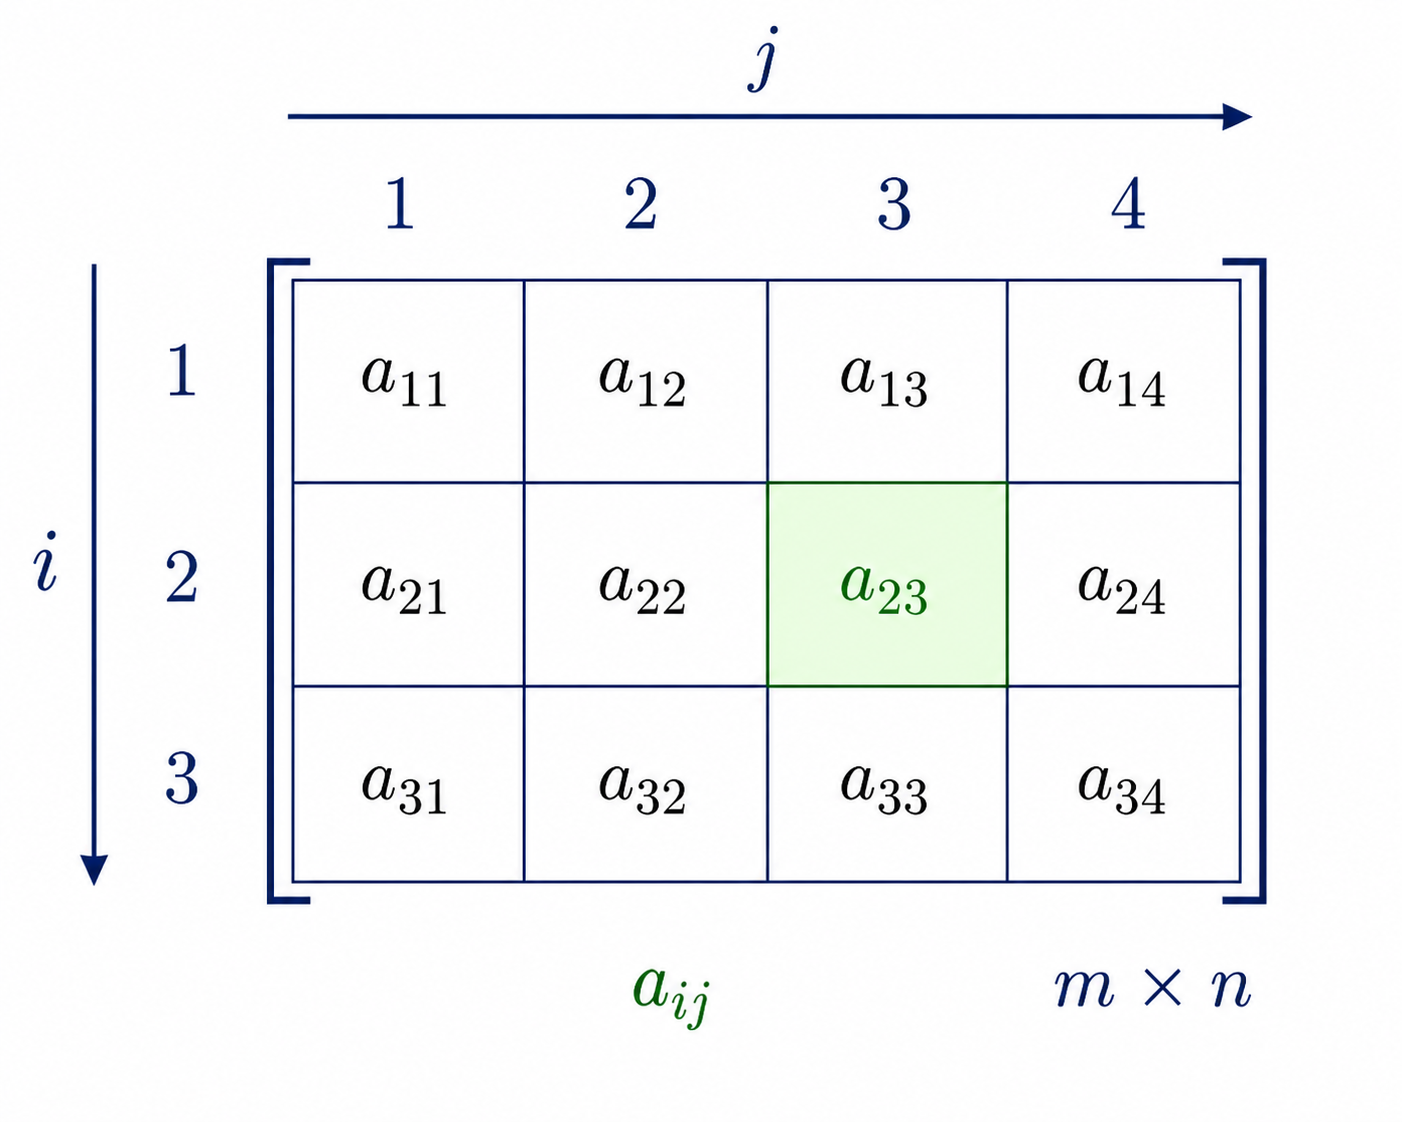
\includegraphics[width=0.62\textwidth]{Figures/png_ready/30-matrix-dimensions-manual.png}
    \caption{แผนภาพแสดงมิติของเมทริกซ์และตำแหน่งสมาชิก}
    \label{fig:matrix-dimensions}
\end{figure}

\begin{definition}[นิยามของเมทริกซ์]
\index{เมทริกซ์!นิยาม}
เมทริกซ์ คือการจัดเรียงข้อมูลในรูปแบบตารางสี่เหลี่ยมผืนผ้า ซึ่งประกอบด้วย $m$ แถว และ $n$ คอลัมน์ เมทริกซ์ขนาด $m \times n$ จะมีสมาชิกทั้งหมด $m \cdot n$ ตัว เขียนแทนด้วย
\[ A_{m \times n} = [a_{ij}]_{m \times n} \]
โดยที่ $a_{ij}$ คือสมาชิกที่อยู่ในแถวที่ $i$ และคอลัมน์ที่ $j$
\end{definition}

\begin{ex}
เมทริกซ์ $A = \begin{pmatrix} 1 & 2 & 3 \\ 4 & 5 & 6 \end{pmatrix}$ มีขนาด $2 \times 3$ (2 แถว 3 คอลัมน์)
\end{ex}
\begin{solution}
$a_{11}=1,\ a_{12}=2,\ a_{13}=3,\ a_{21}=4,\ a_{22}=5,\ a_{23}=6$ \solhere
\end{solution}

\begin{ex}
เมทริกซ์ $B = \begin{pmatrix} 1 & 2 \\ 3 & 4 \\ 5 & 6 \end{pmatrix}$ มีขนาด $3 \times 2$ (3 แถว 2 คอลัมน์)
\end{ex}
\begin{solution}
$B$ มี $3$ แถว ($\begin{psmallmatrix}1&2\end{psmallmatrix},\begin{psmallmatrix}3&4\end{psmallmatrix},\begin{psmallmatrix}5&6\end{psmallmatrix}$) และ $2$ คอลัมน์ $\therefore$ ขนาด $3\times 2$, สมาชิก $3\cdot 2 = 6$ ตัว \solhere
\end{solution}

เมทริกซ์ขนาด $m \times n$ สามารถเขียนในรูปทั่วไปได้ดังนี้

\[
A = \begin{pmatrix}
a_{11} & a_{12} & a_{13} & \cdots & a_{1n} \\
a_{21} & a_{22} & a_{23} & \cdots & a_{2n} \\
a_{31} & a_{32} & a_{33} & \cdots & a_{3n} \\
\vdots & \vdots & \vdots & \ddots & \vdots \\
a_{m1} & a_{m2} & a_{m3} & \cdots & a_{mn}
\end{pmatrix}
\]

\subsection{ประเภทของเมทริกซ์}
เมทริกซ์ในทางคณิตศาสตร์สามารถจำแนกออกได้เป็นหลายประเภทตามลักษณะการจัดเรียงตัวเลขและสมบัติเฉพาะตัวของสมาชิกภายใน โครงสร้างของเมทริกซ์จตุรัส เมทริกซ์ทแยงมุม เมทริกซ์เอกลักษณ์ หรือเมทริกซ์สมมาตร ล้วนมีบทบาทและรูปแบบการดำเนินการที่แตกต่างกันอย่างสิ้นเชิง การวิเคราะห์สมบัติเหล่านี้จะช่วยให้ผู้เรียนสามารถนำประเภทของเมทริกซ์ไปประยุกต์ใช้เพื่อลดความซับซ้อนของการคำนวณในขั้นตอนวิธีประเภทต่าง ๆ ได้อย่างเหมาะสม ดังภาพจำลองประเภทของเมทริกซ์ในรูปที่~\ref{fig:matrix-types}

\begin{figure}[H]
    \centering
    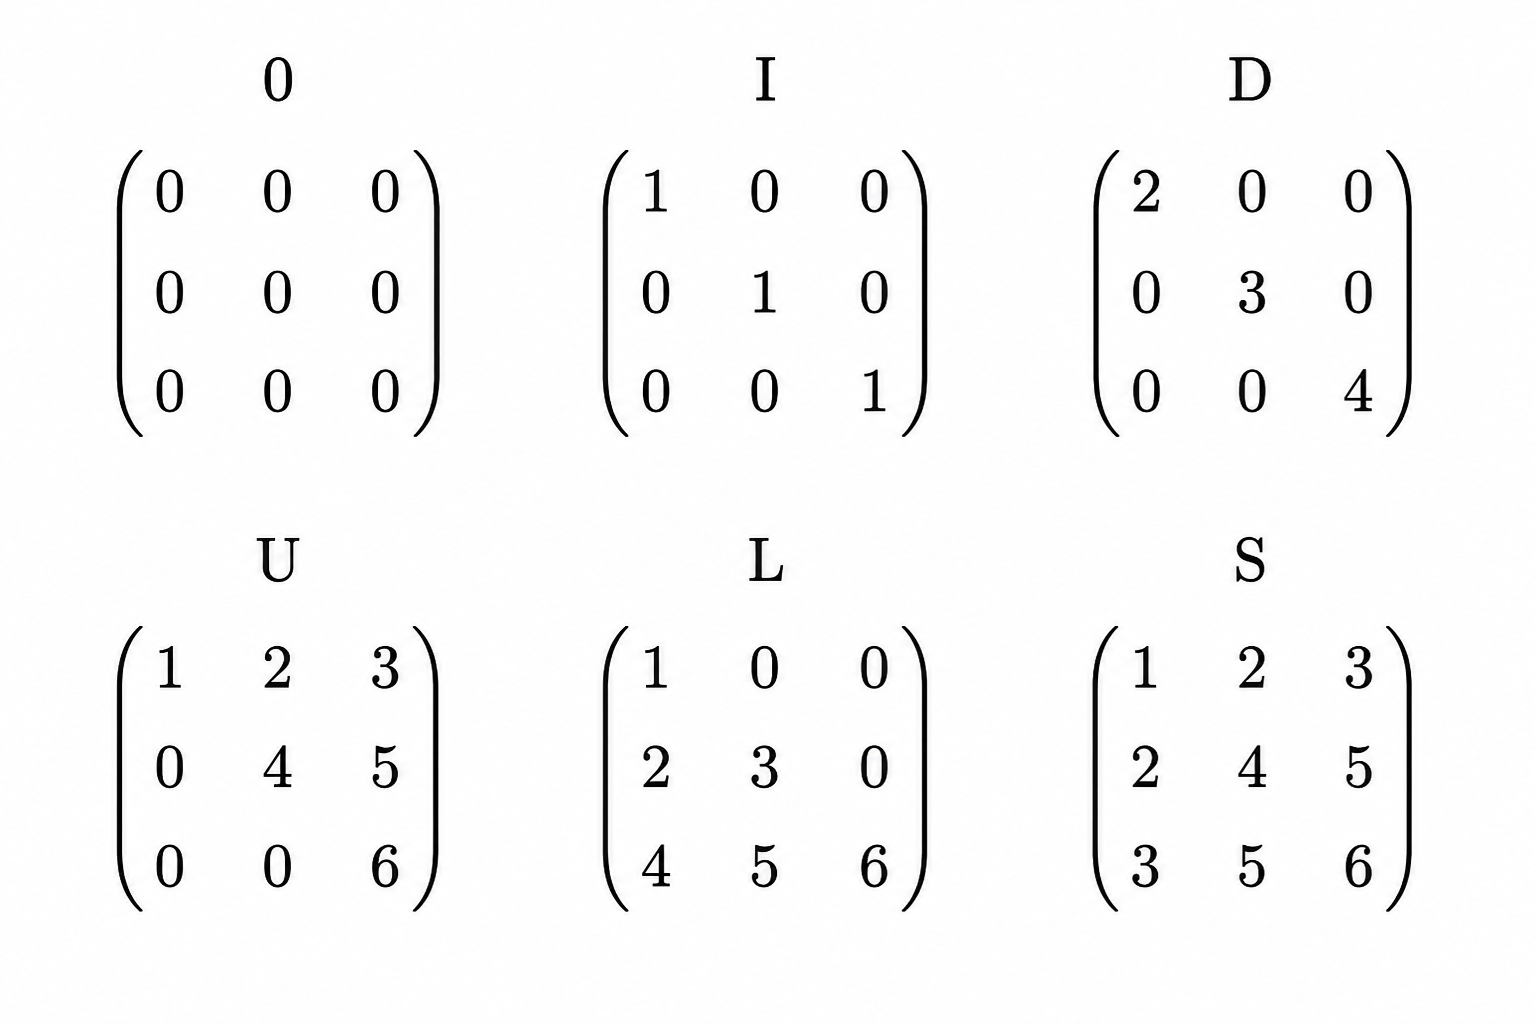
\includegraphics[width=0.62\textwidth]{Figures/png_ready/31-matrix-types-manual.png}
    \caption{แผนภาพแสดงประเภทของเมทริกซ์ที่สำคัญ}
    \label{fig:matrix-types}
\end{figure}

เมทริกซ์แต่ละประเภทมีคุณสมบัติเฉพาะที่แตกต่างกัน การจำแนกประเภทของเมทริกซ์ช่วยให้เข้าใจพฤติกรรมและการประยุกต์ใช้ในบริบททางคณิตศาสตร์และวิทยาการคอมพิวเตอร์ได้ชัดเจนขึ้น โดยเมทริกซ์จตุรัสเป็นประเภทที่สำคัญที่สุดเนื่องจากสามารถคำนวณดีเทอร์มิแนนต์และหาตัวผกผันได้

\begin{definition}[ประเภทของเมทริกซ์]
\index{เมทริกซ์!ประเภท}
เมทริกซ์ในทางคณิตศาสตร์จำแนกตามโครงสร้างและสมบัติเฉพาะของสมาชิกออกเป็นประเภทที่สำคัญ ได้แก่
\end{definition}

\begin{enumerate}
    \item เมทริกซ์ศูนย์ (Zero Matrix) $O_{m \times n}$ คือเมทริกซ์ที่ทุกสมาชิกเป็น 0
    
    \[O = \begin{pmatrix} 0 & 0 & 0 \\ 0 & 0 & 0 \end{pmatrix}\]
    \item เมทริกซ์แถว (Row Matrix) คือเมทริกซ์ที่มีเพียง 1 แถว ($1 \times n$)
    
    \[R = \begin{pmatrix} 1 & 2 & 3 & 4 \end{pmatrix}\]
    \item เมทริกซ์คอลัมน์ (Column Matrix) คือเมทริกซ์ที่มีเพียง 1 คอลัมน์ ($m \times 1$)
    
    \[C = \begin{pmatrix} 1 \\ 2 \\ 3 \end{pmatrix}\]
    \item เมทริกซ์จตุรัส (Square Matrix) คือเมทริกซ์ที่มีจำนวนแถวเท่ากับจำนวนคอลัมน์ ($n \times n$) เรียก $n$ ว่าขนาด (order) ของเมทริกซ์
    
    \[S = \begin{pmatrix} 1 & 2 \\ 3 & 4 \end{pmatrix}\quad (\text{ขนาด } 2 \times 2)\]

    \item เมทริกซ์ทแยงมุม (Diagonal Matrix) คือเมทริกซ์จตุรัสที่สมาชิกนอกเส้นทแยงมุมหลักเป็น 0 ทั้งหมด
    
    \[D = \begin{pmatrix} 1 & 0 & 0 \\ 0 & 2 & 0 \\ 0 & 0 & 3 \end{pmatrix}\]
    \item เมทริกซ์เอกลักษณ์ (Identity Matrix) $I_n$ คือเมทริกซ์ทแยงมุมที่สมาชิกบนเส้นทแยงมุมหลักเป็น 1 ทั้งหมด
    
    \[I_3 = \begin{pmatrix} 1 & 0 & 0 \\ 0 & 1 & 0 \\ 0 & 0 & 1 \end{pmatrix}\]
    \item เมทริกซ์สามเหลี่ยมบน (Upper Triangular Matrix) คือเมทริกซ์จตุรัสที่สมาชิกใต้เส้นทแยงมุมหลักเป็น 0
    
    \[U = \begin{pmatrix} 1 & 2 & 3 \\ 0 & 4 & 5 \\ 0 & 0 & 6 \end{pmatrix}\]
    \item เมทริกซ์สามเหลี่ยมล่าง (Lower Triangular Matrix) คือเมทริกซ์จตุรัสที่สมาชิกเหนือเส้นทแยงมุมหลักเป็น 0
    
    \[L = \begin{pmatrix} 1 & 0 & 0 \\ 2 & 3 & 0 \\ 4 & 5 & 6 \end{pmatrix}\]
    \item เมทริกซ์สมมาตร (Symmetric Matrix) คือเมทริกซ์จตุรัสที่มีคุณสมบัติ $a_{ij} = a_{ji}$ สำหรับทุก $i, j$
    
    \[S = \begin{pmatrix} 1 & 2 & 3 \\ 2 & 4 & 5 \\ 3 & 5 & 6 \end{pmatrix}\]
    \item เมทริกซ์เส้นทแยงมุมเฉียง (Skew-Symmetric Matrix) คือเมทริกซ์จตุรัสที่มีคุณสมบัติ $a_{ij} = -a_{ji}$ สำหรับทุก $i, j$ และ $a_{ii} = 0$
    
    \[K = \begin{pmatrix} 0 & 2 & -3 \\ -2 & 0 & 4 \\ 3 & -4 & 0 \end{pmatrix}\]
\end{enumerate}

\begin{ex}
เมทริกซ์สมมาตรและเมทริกซ์เส้นทแยงมุมเฉียงมีความสำคัญในการประยุกต์ เช่น ในทฤษฎีสถิติ เมทริกซ์ความแปรปรวน (covariance matrix) เป็นเมทริกซ์สมมาตร และในฟิสิกส์ เมทริกซ์เส้นทแยงมุมเฉียงใช้ในการแสดงปริมาณเวกเตอร์
\end{ex}
\begin{solution}
เมทริกซ์สมมาตร ($a_{ij}=a_{ji}$) พบในเมทริกซ์ความแปรปรวน (covariance); เมทริกซ์เส้นทแยงมุมเฉียง ($a_{ij}=-a_{ji},\ a_{ii}=0$) ใช้แทนปริมาณเวกเตอร์ เช่น ทอร์กในฟิสิกส์ $\therefore$ ทั้งสองชนิดช่วยลดความซับซ้อนของการคำนวณ \solhere
\end{solution}

\section{การดำเนินการระหว่างเมทริกซ์}
\label{sec:matrix-operations}
การประยุกต์ใช้เมทริกซ์ในทางปฏิบัติจำเป็นต้องมีนิยามการคำนวณทางพีชคณิตที่สอดคล้องกัน เพื่อแปลงข้อมูลหรือคำนวณค่าผลลัพธ์จากโครงสร้างข้อมูลสองมิตินี้ การดำเนินการพื้นฐานประกอบด้วยความเท่ากันของเมทริกซ์ การบวกและการลบเมทริกซ์ การคูณด้วยปริมาณสเกลาร์ ตลอดจนการคูณกันเองระหว่างสองเมทริกซ์ และการสลับเปลี่ยนแถวเป็นคอลัมน์ การดำเนินการแต่ละประเภทมีกฎเกณฑ์ เงื่อนไขข้อกำหนด และสมบัติทางคณิตศาสตร์ที่ผู้เรียนต้องเข้าใจเพื่อหลีกเลี่ยงความเข้าใจผิดในการวิเคราะห์ระบบ ดังรายละเอียดเชิงลึกและเงื่อนไขการคำนวณต่อไปนี้

\subsection{ความเท่ากันของเมทริกซ์}
ความสัมพันธ์ระดับพื้นฐานที่สุดระหว่างสองเมทริกซ์คือความเท่ากัน ซึ่งกำหนดเงื่อนไขทางโครงสร้างที่เข้มงวดสำหรับการเปรียบเทียบค่าข้อมูลในแต่ละตำแหน่ง การตรวจสอบความเท่ากันจะทำได้ก็ต่อเมื่อเมทริกซ์ทั้งสองมีมิติที่สอดคล้องกันอย่างสมบูรณ์ และค่าสมาชิกในทุกตำแหน่งตรงกันทุกประการ สมบัตินี้มักถูกนำไปใช้ในขั้นตอนวิธีการจับคู่ข้อมูล (Pattern Matching) และการคำนวณค่าตัวแปรในระบบสมการเชิงเส้น ดังนิยามต่อไปนี้
\begin{definition}[ความเท่ากันของเมทริกซ์]
\index{ความเท่ากันของเมทริกซ์!นิยาม}
เมทริกซ์ $A = [a_{ij}]$ และ $B = [b_{ij}]$ ขนาด $m \times n$ เท่ากัน ก็ต่อเมื่อ
\[ a_{ij} = b_{ij} \quad \forall i \in \{1,\ldots,m\}, j \in \{1,\ldots,n\} \]
\end{definition}

\begin{ex}
ถ้า $\begin{pmatrix} x & 2 \\ 3 & y \end{pmatrix} = \begin{pmatrix} 1 & 2 \\ 3 & 4 \end{pmatrix}$ แล้ว $x = 1$ และ $y = 4$
\end{ex}
\begin{solution}
\begin{align*}
(1,1):\ & x = 1\\
(2,2):\ & y = 4
\end{align*}
$\therefore x=1,\ y=4$ \solhere
\end{solution}

\subsection{การบวกและการลบเมทริกซ์}
การดำเนินการเพิ่มหรือลดระดับค่าของข้อมูลในตารางสองมิติมักทำผ่านการบวกและการลบเมทริกซ์ โดยมีเงื่อนไขพื้นฐานว่าเมทริกซ์คู่กรณีจะต้องมีขนาดมิติเท่ากันทุกประการเพื่อจะนำสมาชิกในตำแหน่งเดียวกันมาทำปฏิกิริยากันทางพีชคณิต หากขนาดมิติไม่เท่ากันจะไม่สามารถดำเนินการได้เนื่องจากจะไม่มีคู่สมาชิกมารองรับการรวมค่า ซึ่งผลลัพธ์จากการดำเนินการจะได้เมทริกซ์ใหม่ที่มีมิติคงเดิม ดังอธิบายตามบทนิยามและตัวอย่างต่อไปนี้

\begin{definition}[การบวกและการลบเมทริกซ์]
\index{การบวกเมทริกซ์!นิยาม}
\index{การลบเมทริกซ์!นิยาม}
กำหนดเมทริกซ์ $A = [a_{ij}]$ และ $B = [b_{ij}]$ ขนาด $m \times n$ การบวกและการลบเมทริกซ์กำหนดโดย
\[ A + B = [a_{ij} + b_{ij}] \quad\text{และ}\quad A - B = [a_{ij} - b_{ij}] \]
\end{definition}

หมายเหตุ: เมทริกซ์สองเมทริกซ์จะบวกหรือลบกันได้ก็ต่อเมื่อมีขนาดเท่ากัน

\begin{ex}
จงคำนวณผลลัพธ์ของการบวกและการลบเมทริกซ์ต่อไปนี้
\[
\begin{pmatrix} 1 & 2 & 3 \\ 4 & 5 & 6 \end{pmatrix} + \begin{pmatrix} 1 & 1 & 1 \\ 2 & 2 & 2 \end{pmatrix} = \;?
\]

\[
\begin{pmatrix} 5 & 6 \\ 7 & 8 \end{pmatrix} - \begin{pmatrix} 1 & 2 \\ 3 & 4 \end{pmatrix} = \;?
\]
\end{ex}
\begin{solution}
\begin{align*}
\begin{pmatrix} 1 & 2 & 3 \\ 4 & 5 & 6 \end{pmatrix} + \begin{pmatrix} 1 & 1 & 1 \\ 2 & 2 & 2 \end{pmatrix} &= \begin{pmatrix} 2 & 3 & 4 \\ 6 & 7 & 8 \end{pmatrix}\\
\begin{pmatrix} 5 & 6 \\ 7 & 8 \end{pmatrix} - \begin{pmatrix} 1 & 2 \\ 3 & 4 \end{pmatrix} &= \begin{pmatrix} 4 & 4 \\ 4 & 4 \end{pmatrix}
\end{align*}
\solhere
\end{solution}

\begin{ex}[สมบัติของการบวกเมทริกซ์]
สำหรับเมทริกซ์ $A, B, C$ ขนาด $m \times n$:
\begin{enumerate}
    \item $A + B = B + A$ \hfill (Commutative Law)
    \item $(A + B) + C = A + (B + C)$ \hfill (Associative Law)
    \item $A + O = A$ \hfill (Identity Law, $O$ คือเมทริกซ์ศูนย์)
    \item $A + (-A) = O$ \hfill (Inverse Law)
    \item $A - B = A + (-B)$
\end{enumerate}
\end{ex}
\begin{solution}
ทุกสมบัติลดรูปเป็นสมบัติการบวกจำนวนจริงรายตำแหน่ง
\begin{align*}
[A+B]_{ij} &= a_{ij}+b_{ij} = b_{ij}+a_{ij} = [B+A]_{ij}\\
[(A+B)+C]_{ij} &= a_{ij}+b_{ij}+c_{ij} = [A+(B+C)]_{ij}\\
[A+O]_{ij} &= a_{ij}+0 = a_{ij}\\
[A+(-A)]_{ij} &= a_{ij}-a_{ij} = 0
\end{align*}
$\therefore$ สลับที่ เปลี่ยนหมู่ เอกลักษณ์ ตรงข้าม เป็นจริง และ $A-B=A+(-B)$ \solhere
\end{solution}

\begin{ex}
การลบเมทริกซ์ไม่มีสมบัติการสลับที่ กล่าวคือ $A - B \neq B - A$ โดยทั่วไป
\end{ex}
\begin{solution}
ให้ $A = \begin{pmatrix} 1 & 2 \\ 3 & 4 \end{pmatrix}$, $B = \begin{pmatrix} 5 & 6 \\ 7 & 8 \end{pmatrix}$
\begin{align*}
A-B &= \begin{pmatrix} -4 & -4 \\ -4 & -4 \end{pmatrix}, \qquad
B-A = \begin{pmatrix} 4 & 4 \\ 4 & 4 \end{pmatrix}
\end{align*}
$\therefore A-B \neq B-A$ (การลบไม่มีสมบัติสลับที่) \solhere
\end{solution}

\subsection{การคูณเมทริกซ์ด้วยสเกลาร์}
การปรับขนาดหรือการขยายค่าของสมาชิกทุกตัวในเมทริกซ์อย่างสม่ำเสมอทำได้ด้วยการคูณด้วยปริมาณสเกลาร์หรือตัวเลขคงที่จำนวนจริง ค่าสเกลาร์จะถูกกระจายไปคูณกับสมาชิกในทุกตำแหน่งของเมทริกซ์อย่างไม่มีข้อยกเว้น ส่งผลให้ลักษณะเชิงโครงสร้างยังคงเดิมแต่มีขนาดของปริมาณเปลี่ยนแปลงไปตามสัดส่วนของสเกลาร์นั้น การดำเนินการนี้พบได้ทั่วไปในวิชากราฟิกส์คอมพิวเตอร์เมื่อมีการขยายภาพหรือปรับแต่งระดับความเข้มสี ดังรายละเอียดตามบทนิยามต่อไปนี้

\begin{definition}[การคูณเมทริกซ์ด้วยสเกลาร์]
\index{การคูณเมทริกซ์ด้วยสเกลาร์!นิยาม}
กำหนดเมทริกซ์ $A = [a_{ij}]$ ขนาด $m \times n$ และสเกลาร์ $c$ (ค่าคงตัวจำนวนจริง) การคูณสเกลาร์ $cA$ คือเมทริกซ์
\[ cA = [c \cdot a_{ij}] \]
\end{definition}

\begin{ex}
\[
3 \cdot \begin{pmatrix} 1 & 2 \\ 3 & 4 \end{pmatrix} = \begin{pmatrix} 3 & 6 \\ 9 & 12 \end{pmatrix}
\]
\end{ex}
\begin{solution}
\[
3\begin{pmatrix} 1 & 2 \\ 3 & 4 \end{pmatrix} = \begin{pmatrix} 3\cdot1 & 3\cdot2 \\ 3\cdot3 & 3\cdot4 \end{pmatrix} = \begin{pmatrix} 3 & 6 \\ 9 & 12 \end{pmatrix}
\]
\solhere
\end{solution}

\begin{ex}[สมบัติของการคูณสเกลาร์]
สำหรับเมทริกซ์ $A, B$ และสเกลาร์ $c, d$:
\begin{enumerate}
    \item $c(A + B) = cA + cB$ \hfill (Distributive Law)
    \item $(c + d)A = cA + dA$ \hfill (Distributive Law)
    \item $c(dA) = (cd)A$ \hfill (Associative Law)
    \item $1A = A$ \hfill (Identity Law)
    \item $0A = O$ \hfill (Zero Law)
\end{enumerate}
\end{ex}
\begin{solution}
ทุกสมบัติลดรูปเป็นสมบัติการคูณ/บวกจำนวนจริงรายตำแหน่ง
\begin{align*}
[c(A+B)]_{ij} &= c(a_{ij}+b_{ij}) = ca_{ij}+cb_{ij} = [cA+cB]_{ij}\\
[(c+d)A]_{ij} &= (c+d)a_{ij} = ca_{ij}+da_{ij} = [cA+dA]_{ij}\\
[c(dA)]_{ij} &= c(d\,a_{ij}) = (cd)a_{ij} = [(cd)A]_{ij}\\
[1A]_{ij} &= a_{ij}, \qquad [0A]_{ij} = 0
\end{align*}
$\therefore$ การกระจาย เปลี่ยนหมู่ เอกลักษณ์ ศูนย์ เป็นจริงทั้งหมด \solhere
\end{solution}

\subsection{การคูณเมทริกซ์ด้วยเมทริกซ์}
การดำเนินการคูณระหว่างเมทริกซ์ด้วยกันเองมีมิติความซับซ้อนที่สูงกว่าการดำเนินการอื่น ๆ เนื่องจากผลลัพธ์ไม่ได้เกิดจากการนำตำแหน่งเดียวกันมาคูณกันโดยตรง แต่ต้องอาศัยการจับคู่ผลรวมคูณสะสมระหว่างแถวของเมทริกซ์ตัวหน้ากับคอลัมน์ของเมทริกซ์ตัวหลัง เงื่อนไขสำคัญคือจำนวนคอลัมน์ของตัวตั้งจะต้องเท่ากับจำนวนแถวของตัวคูณพอดี จึงจะสามารถเกิดผลคูณสอดคล้อง (Conformable) ได้ การคูณเมทริกซ์ถูกใช้แสดงความเชื่อมโยงเชิงเส้นในแบบจำลองการแปลงรูปพิกเซลและโครงข่ายประสาทเทียม ดังแสดงลักษณะการทำงานในรูปที่~\ref{fig:matrix-multiplication}

\begin{figure}[H]
    \centering
    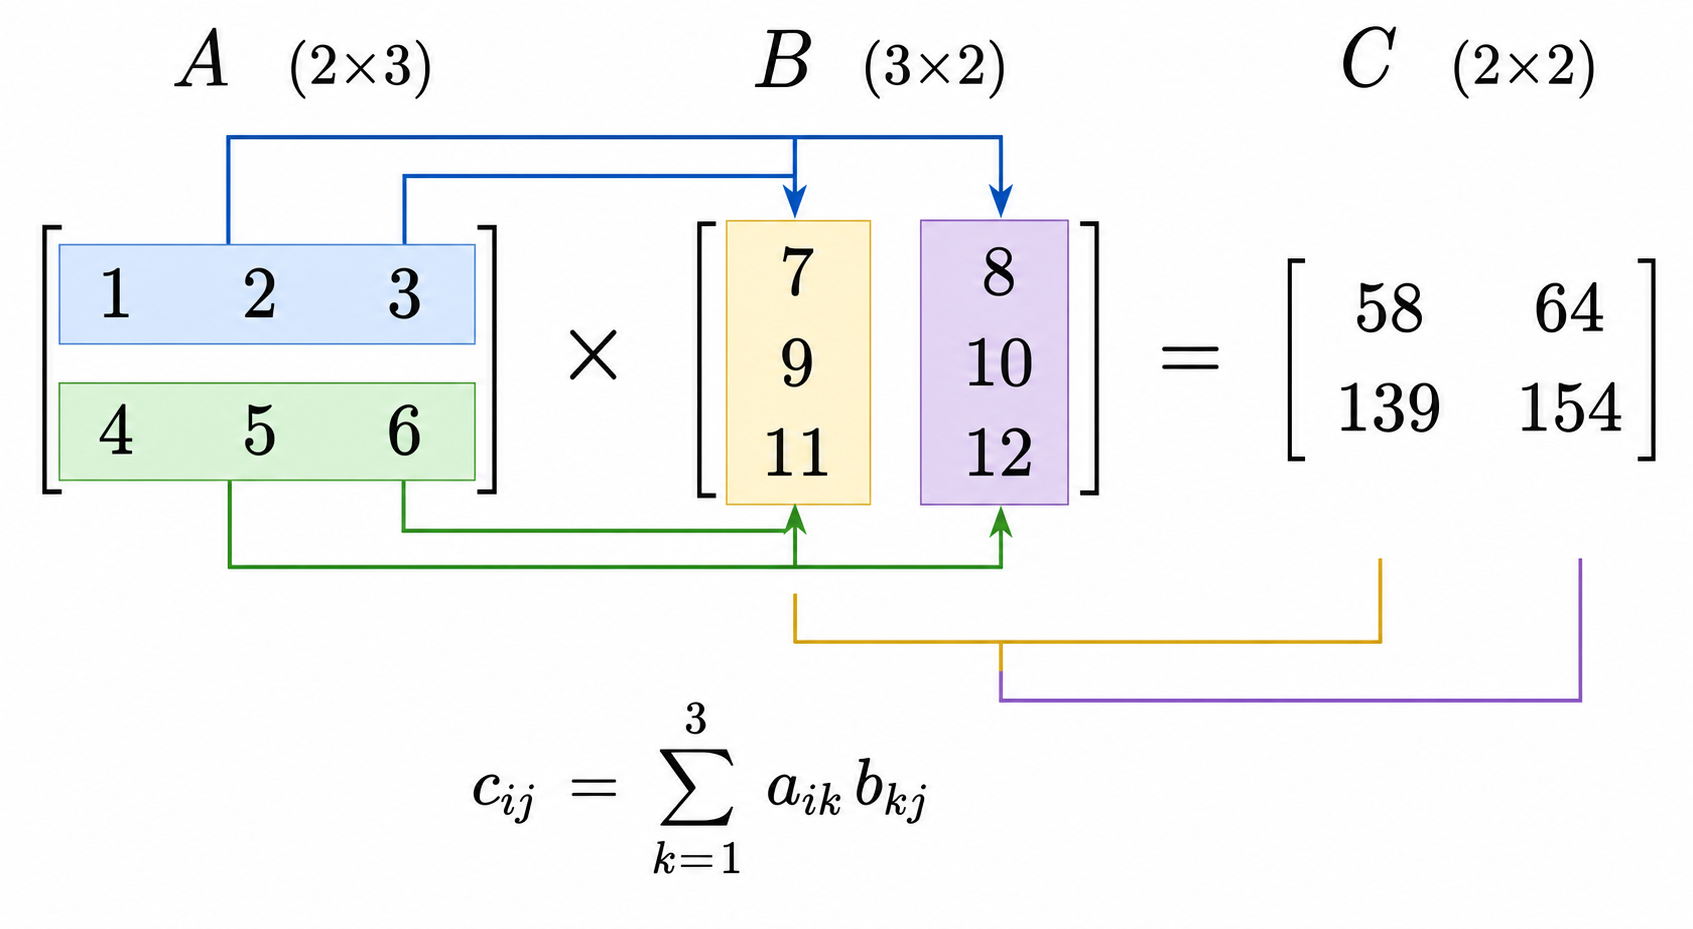
\includegraphics[width=0.62\textwidth]{Figures/png_ready/32-matrix-multiplication-manual.png}
    \caption{แผนภาพแสดงการคูณแถวของเมทริกซ์กับหลักของเมทริกซ์}
    \label{fig:matrix-multiplication}
\end{figure}

การคูณเมทริกซ์เป็นการดำเนินการที่ซับซ้อนกว่าการบวกและการคูณสเกลาร์ สมาชิกของเมทริกซ์ผลคูณคำนวณจากผลรวมของผลคูณของสมาชิกในแถวของเมทริกซ์ตัวแรกกับสมาชิกในคอลัมน์ของเมทริกซ์ตัวที่สอง การคูณเมทริกซ์สามารถมองได้ว่าเป็นการแทนการแปลงเชิงเส้น (linear transformation) ซึ่งใช้อย่างกว้างขวางในคณิตศาสตร์และวิทยาการคอมพิวเตอร์

\begin{definition}[การคูณเมทริกซ์ด้วยเมทริกซ์]
\index{การคูณเมทริกซ์!นิยาม}
กำหนดเมทริกซ์ $A = [a_{ij}]$ ขนาด $m \times n$ และเมทริกซ์ $B = [b_{jk}]$ ขนาด $n \times p$ ผลคูณ $AB$ จะได้เมทริกซ์ $C = [c_{ik}]$ ขนาด $m \times p$ โดยสมาชิกในแถวที่ $i$ คอลัมน์ที่ $k$ คือ
\[
c_{ik} = a_{i1}b_{1k} + a_{i2}b_{2k} + a_{i3}b_{3k} + \cdots + a_{in}b_{nk} = \sum_{j=1}^{n} a_{ij}b_{jk}
\]
\end{definition}

หมายเหตุ การคูณ $AB$ กระทำได้ก็ต่อเมื่อจำนวนคอลัมน์ของ $A$ เท่ากับจำนวนแถวของ $B$ (เรียกว่า conformable)

\begin{thrm}[สมบัติของการคูณเมทริกซ์]
สำหรับเมทริกซ์ $A, B, C$ ที่ขนาดเหมาะสม และสเกลาร์ $c$ การคูณเมทริกซ์มีสมบัติดังต่อไปนี้
\begin{enumerate}
    \item $(AB)C = A(BC)$ \hfill (Associative Law)
    \item $A(B + C) = AB + AC$ \hfill (Left Distributive Law)
    \item $(A + B)C = AC + BC$ \hfill (Right Distributive Law)
    \item $AI = IA = A$ \hfill (Identity Law, $I$ คือเมทริกซ์เอกลักษณ์)
    \item $c(AB) = (cA)B = A(cB)$ \hfill (Scalar Multiplication)
    \item $(AB)^T = B^T A^T$ \hfill (Transpose of Product)
\end{enumerate}
\end{thrm}

\begin{thrm}
สำหรับเมทริกซ์ $A$ และ $B$ ที่สามารถคูณกันได้ จะได้ว่า $(AB)^T = B^T A^T$
\end{thrm}

\begin{proof}
การพิสูจน์สมบัติ $(AB)^T = B^T A^T$ พิจารณาเปรียบเทียบสมาชิกในตำแหน่ง $(k,i)$ เป็นขั้นตอนดังนี้:
\begin{enumerate}[label=\textbf{\arabic*.}]
    \item \textbf{กำหนดเมทริกซ์ผลคูณ:} ให้ $A = [a_{ij}]$ และ $B = [b_{jk}]$ ให้ $C = AB$ เป็นเมทริกซ์ผลคูณ โดยมีสมาชิกตำแหน่ง $(i,k)$ คือ
    \[ c_{ik} = \sum_{j} a_{ij}b_{jk} \]
    
    \item \textbf{หาทรานสโพสของผลคูณ ($C^T$):} จากนิยามทรานสโพส สมาชิกในตำแหน่ง $(k,i)$ ของ $C^T$ คือ
    \[ (C^T)_{ki} = C_{ik} = \sum_{j} a_{ij}b_{jk} \]
    
    \item \textbf{หาผลคูณของทรานสโพสย้อนกลับ ($B^T A^T$):} สมาชิกในตำแหน่ง $(k,i)$ ของ $B^T A^T$ คือ
    \[ (B^T A^T)_{ki} = \sum_{j} (B^T)_{kj} (A^T)_{ji} = \sum_{j} b_{jk} a_{ij} \]
    
    \item \textbf{สรุปผลการสลับที่การคูณ:} เนื่องจาก $a_{ij}b_{jk} = b_{jk}a_{ij}$ เป็นสเกลาร์ที่สลับที่การคูณได้ ทำให้ $(C^T)_{ki} = (B^T A^T)_{ki}$ สำหรับทุกตำแหน่ง
\end{enumerate}
ดังนั้นจึงสรุปได้ว่า $(AB)^T = B^T A^T$
\end{proof}

\begin{ex}
จงหาผลคูณ $AB$ เมื่อ
\[
A = \begin{pmatrix} 1 & 2 \\ 3 & 4 \end{pmatrix}, \quad B = \begin{pmatrix} 5 & 6 \\ 7 & 8 \end{pmatrix}
\]
\end{ex}

\begin{solution}
$A_{2\times2}B_{2\times2}$ กระทำได้ ($c_{ik}=\sum_j a_{ij}b_{jk}$)
\begin{align*}
AB &= \begin{pmatrix} (1)(5)+(2)(7) & (1)(6)+(2)(8) \\ (3)(5)+(4)(7) & (3)(6)+(4)(8) \end{pmatrix}\\
&= \begin{pmatrix} 19 & 22 \\ 43 & 50 \end{pmatrix}
\end{align*}
\solhere
\end{solution}

\begin{ex}
จงคำนวณผลคูณ $AB$ และ $BA$ เมื่อ
\[
A = \begin{pmatrix} 1 & 2 & 3 \end{pmatrix}, \quad B = \begin{pmatrix} 4 \\ 5 \\ 6 \end{pmatrix}
\]
แล้วสังเกตว่าการคูณเมทริกซ์ไม่มีสมบัติสลับที่
\end{ex}
\begin{solution}
\begin{align*}
AB &= \begin{pmatrix} 1 & 2 & 3 \end{pmatrix}\begin{pmatrix} 4 \\ 5 \\ 6 \end{pmatrix} = [1(4)+2(5)+3(6)] = [32]\\
BA &= \begin{pmatrix} 4 \\ 5 \\ 6 \end{pmatrix}\begin{pmatrix} 1 & 2 & 3 \end{pmatrix} = \begin{pmatrix} 4 & 8 & 12 \\ 5 & 10 & 15 \\ 6 & 12 & 18 \end{pmatrix}
\end{align*}
$\therefore AB \neq BA$ (การคูณเมทริกซ์ไม่มีสมบัติสลับที่) \solhere
\end{solution}

\begin{ex}
จงหาผลคูณ $AB$ โดยที่ $A = \begin{pmatrix} 2 & 3 \\ 1 & 4 \end{pmatrix}$ และ $B = \begin{pmatrix} 5 & 2 \\ 1 & 6 \end{pmatrix}$
\end{ex}

\begin{solution}
\begin{align*}
AB &= \begin{pmatrix} (2)(5)+(3)(1) & (2)(2)+(3)(6) \\ (1)(5)+(4)(1) & (1)(2)+(4)(6) \end{pmatrix}\\
&= \begin{pmatrix} 13 & 22 \\ 9 & 26 \end{pmatrix}
\end{align*}
\solhere
\end{solution}

\begin{ex}
การคูณเมทริกซ์ไม่มีสมบัติการสลับที่ กล่าวคือ $AB \neq BA$ โดยทั่วไป นอกจากนี้ $AB = O$ ไม่ได้หมายความว่า $A = O$ หรือ $B = O$
\end{ex}
\begin{solution}
\textbf{ไม่สลับที่:} ให้ $A = \begin{pmatrix} 1 & 2 \\ 3 & 4 \end{pmatrix}$, $B = \begin{pmatrix} 5 & 6 \\ 7 & 8 \end{pmatrix}$
\[
AB = \begin{pmatrix} 19 & 22 \\ 43 & 50 \end{pmatrix} \neq \begin{pmatrix} 23 & 34 \\ 31 & 46 \end{pmatrix} = BA
\]
\textbf{$AB=O$ ไม่บังคับ $A=O$ หรือ $B=O$:} ให้ $A = \begin{pmatrix} 1 & 1 \\ 1 & 1 \end{pmatrix}$, $B = \begin{pmatrix} 1 & -1 \\ -1 & 1 \end{pmatrix}$
\[
AB = \begin{pmatrix} 0 & 0 \\ 0 & 0 \end{pmatrix} = O \quad\text{แต่}\quad A,B \neq O
\]
\solhere
\end{solution}

\begin{ex}[สมบัติของการคูณเมทริกซ์]
สำหรับเมทริกซ์ $A, B, C$ ที่ขนาดเหมาะสม และสเกลาร์ $c$:
\begin{enumerate}
    \item $(AB)C = A(BC)$ \hfill (Associative Law)
    \item $A(B + C) = AB + AC$ \hfill (Left Distributive Law)
    \item $(A + B)C = AC + BC$ \hfill (Right Distributive Law)
    \item $AI = IA = A$ \hfill (Identity Law, $I$ คือเมทริกซ์เอกลักษณ์)
    \item $c(AB) = (cA)B = A(cB)$ \hfill (Scalar Multiplication)
    \item $(AB)^T = B^T A^T$ \hfill (Transpose of Product)
\end{enumerate}
\end{ex}
\begin{solution}
สมบัติทั้งหกพิสูจน์ได้จากนิยาม $[AB]_{ik}=\sum_j a_{ij}b_{jk}$ และสมบัติของผลบวก/ผลคูณจำนวนจริง เช่น การเปลี่ยนหมู่
\[
[(AB)C]_{i\ell} = \sum_{j,k} a_{ij}b_{jk}c_{k\ell} = [A(BC)]_{i\ell}
\]
และการแจกแจง $A(B+C)=AB+AC$, เอกลักษณ์ $AI=IA=A$; ส่วน $(AB)^T=B^TA^T$ พิสูจน์ในตัวอย่างถัดไป $\therefore$ ทุกสมบัติเป็นจริง \solhere
\end{solution}

\begin{ex}
พิสูจน์ $(AB)^T = B^T A^T$
\end{ex}
\begin{solution}
\begin{align*}
[(AB)^T]_{ki} &= [AB]_{ik} = \sum_{j} a_{ij}b_{jk}\\
[B^T A^T]_{ki} &= \sum_{j} [B^T]_{kj}[A^T]_{ji} = \sum_{j} b_{jk}a_{ij} = \sum_{j} a_{ij}b_{jk}
\end{align*}
$\therefore [(AB)^T]_{ki} = [B^TA^T]_{ki}$ ทุก $(k,i)$ จึง $(AB)^T = B^TA^T$ \solhere
\end{solution}

\subsection{เมทริกซ์สลับเปลี่ยน (Transpose)}
เมทริกซ์สลับเปลี่ยนเป็นการดำเนินการพื้นฐานที่สลับโครงสร้างทิศทางของข้อมูล โดยเปลี่ยนแถวของเมทริกซ์ให้กลายเป็นคอลัมน์ และเปลี่ยนคอลัมน์ของเมทริกซ์ให้กลายเป็นแถวตามลำดับ สมบัตินี้ช่วยอำนวยความสะดวกในการวิเคราะห์สมบัติเชิงพีชคณิตเชิงเส้นเชิงลึก เช่น การคำนวณหาสมมาตรของเมทริกซ์ความแปรปรวนร่วมเกี่ยว ตลอดจนการหาตัวผกผันในปริภูมิของเมทริกซ์เชิงตั้งฉาก (Orthogonal Matrix) ดังรายละเอียดตามนิยามต่อไปนี้

\begin{definition}[เมทริกซ์สลับเปลี่ยน]
\index{เมทริกซ์สลับเปลี่ยน!นิยาม}
เมทริกซ์สลับเปลี่ยน ของเมทริกซ์ $A = [a_{ij}]$ ขนาด $m \times n$ คือเมทริกซ์
\[ A^T = [a_{ji}]_{n \times m} \]
ที่เกิดจากการสลับแถวเป็นคอลัมน์
\end{definition}

\begin{ex}
จงหา transpose ของเมทริกซ์ $A = \begin{pmatrix} 1 & 2 & 3 \\ 4 & 5 & 6 \end{pmatrix}$
\end{ex}
\begin{solution}
\[
A = \begin{pmatrix} 1 & 2 & 3 \\ 4 & 5 & 6 \end{pmatrix} \Rightarrow A^T = \begin{pmatrix} 1 & 4 \\ 2 & 5 \\ 3 & 6 \end{pmatrix} \quad (\text{ขนาด } 3\times 2)
\]
\solhere
\end{solution}

\begin{ex}[สมบัติของ Transpose]
สำหรับเมทริกซ์ $A, B$:
\begin{enumerate}
    \item $(A^T)^T = A$
    \item $(A + B)^T = A^T + B^T$
    \item $(cA)^T = cA^T$
    \item $(AB)^T = B^T A^T$
\end{enumerate}
\end{ex}
\begin{solution}
ทุกสมบัติตามนิยาม $[A^T]_{ij}=a_{ji}$
\begin{align*}
[(A^T)^T]_{ij} &= [A^T]_{ji} = a_{ij} \Rightarrow (A^T)^T = A\\
[(A+B)^T]_{ij} &= a_{ji}+b_{ji} = [A^T+B^T]_{ij}\\
[(cA)^T]_{ij} &= c\,a_{ji} = [cA^T]_{ij}
\end{align*}
$\therefore$ ทั้งสามเป็นจริง และ $(AB)^T=B^TA^T$ (พิสูจน์แล้วข้างต้น) \solhere
\end{solution}

\begin{thrm}
เมทริกซ์จตุรัส $A$ เป็นสมมาตร (Symmetric) ก็ต่อเมื่อ $A^T = A$ และเป็นเส้นทแยงมุมเฉียง (Skew-Symmetric) ก็ต่อเมื่อ $A^T = -A$
\end{thrm}

\begin{thrm}
ทุกเมทริกซ์จตุรัส $A$ สามารถเขียนได้ในรูปผลบวกของเมทริกซ์สมมาตรและเมทริกซ์เส้นทแยงมุมเฉียง ดังนี้

\[
A = \frac{1}{2}(A + A^T) + \frac{1}{2}(A - A^T)
\]
โดยที่ $\frac{1}{2}(A + A^T)$ เป็นเมทริกซ์สมมาตร เนื่องจาก $(\frac{1}{2}(A + A^T))^T = \frac{1}{2}(A + A^T)$ และ $\frac{1}{2}(A - A^T)$ เป็นเมทริกซ์เส้นทแยงมุมเฉียง เนื่องจาก $(\frac{1}{2}(A - A^T))^T = -\frac{1}{2}(A - A^T)$
\end{thrm}

\section{ดีเทอร์มิแนนต์ (Determinants)}
\label{sec:determinants}
ดีเทอร์มิแนนต์เป็นคุณลักษณะเฉพาะเชิงตัวเลขที่สำคัญยิ่งของเมทริกซ์จตุรัส ซึ่งทำหน้าที่สะท้อนสมบัติการเปลี่ยนขนาดของปริมาตรเมื่อมองเมทริกซ์ในฐานะการแปลงเชิงเส้น ค่าดีเทอร์มิแนนต์ช่วยระบุว่าเมทริกซ์นั้นมีตัวผกผันหรือไม่ และใช้เป็นค่าตัวหารหลักในสูตรการคำนวณต่าง ๆ ของการแก้ระบบสมการเชิงเส้น ในหัวข้อนี้ผู้เรียนจะได้ศึกษาความหมาย บทนิยามเชิงเลขคณิต สมบัติต่าง ๆ รวมถึงวิธีการคำนวณสำหรับเมทริกซ์ขนาดต่าง ๆ ดังต่อไปนี้

\subsection{นิยามของดีเทอร์มิแนนต์}
นิยามเชิงคณิตศาสตร์ของดีเทอร์มิแนนต์เริ่มต้นจากกรณีพื้นฐานขนาดมิติต่ำ ซึ่งช่วยสร้างความเข้าใจเชิงกลไกเกี่ยวกับการถ่วงน้ำหนักและการหักล้างกันของสมาชิกในทแยงมุมหลักและทแยงมุมรอง แผนภาพแสดงทิศทางการคูณตัวเลขทแยงมุมขึ้นลงสำหรับเมทริกซ์ขนาดสองคูณสอง จะเป็นรากฐานสำหรับสูตรการคำนวณที่ซับซ้อนขึ้นในมิติสูง ดังอธิบายและจำลองรายละเอียดในรูปที่~\ref{fig:determinant-2x2}

\begin{figure}[H]
    \centering
    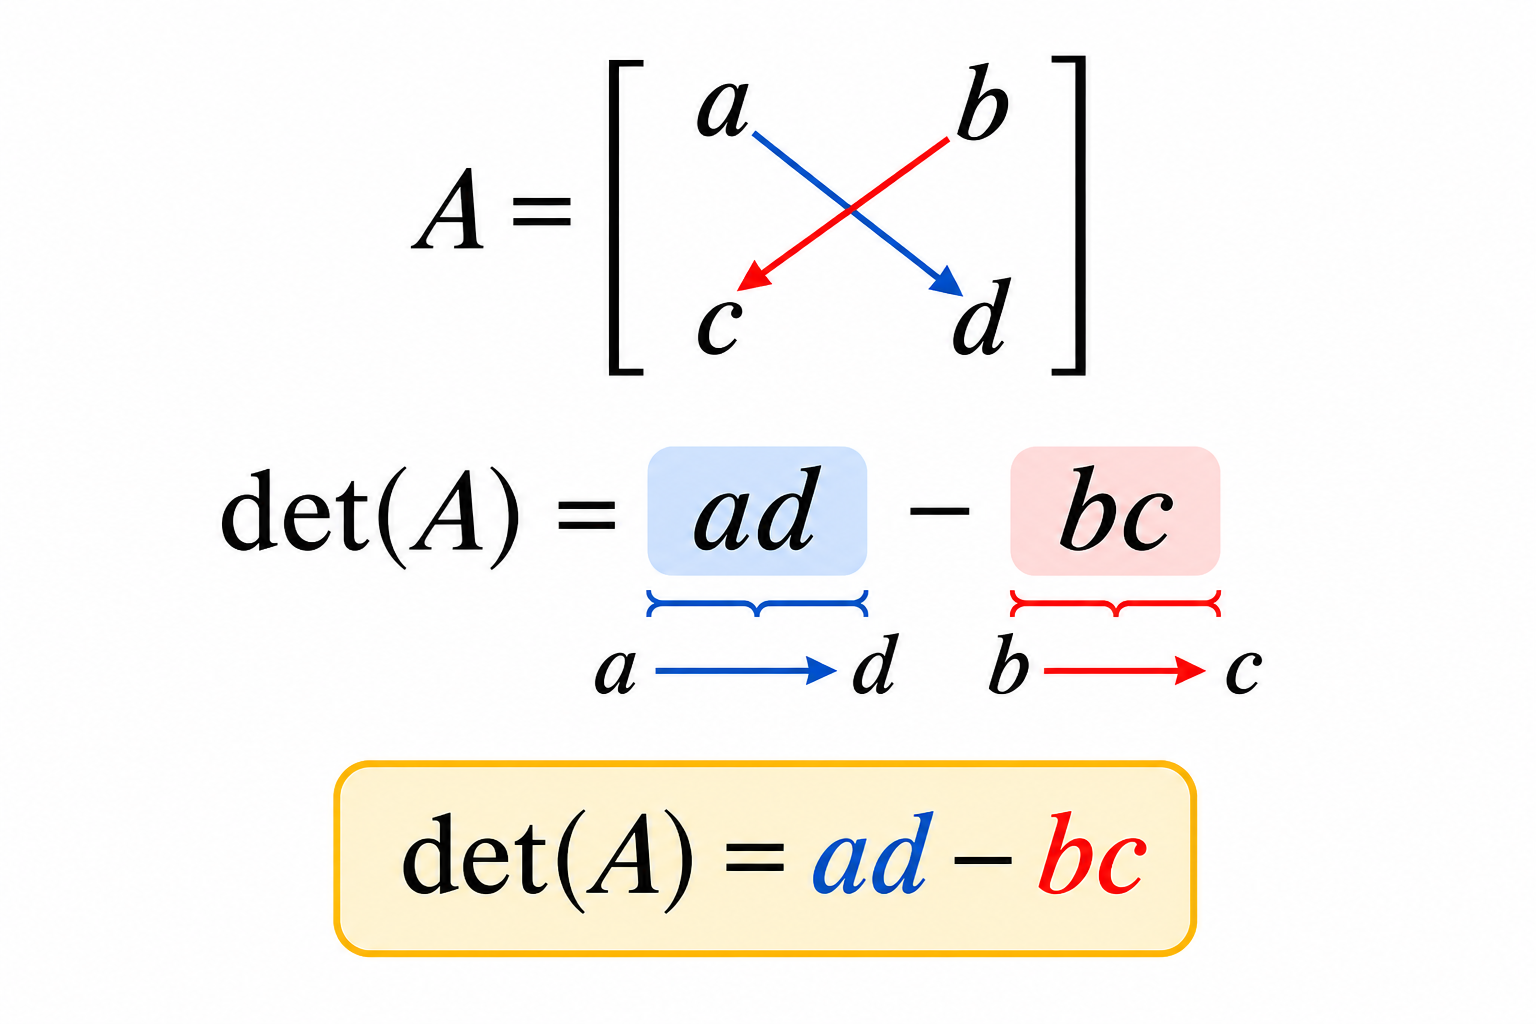
\includegraphics[width=0.62\textwidth]{Figures/png_ready/33-determinant-2x2-manual.png}
    \caption{แผนภาพแสดงดีเทอร์มิแนนต์ของเมทริกซ์ $2\times2$}
    \label{fig:determinant-2x2}
\end{figure}


\begin{definition}[ดีเทอร์มิแนนต์]
\index{ดีเทอร์มิแนนต์!นิยาม}
ดีเทอร์มิแนนต์ ของเมทริกซ์จตุรัส $A$ ขนาด $n \times n$ เขียนแทนด้วย $\det(A)$ หรือ $|A|$
\end{definition}

\begin{definition}[ดีเทอร์มิแนนต์ของเมทริกซ์ขนาดเล็ก]
ดีเทอร์มิแนนต์ของเมทริกซ์จตุรัสนิยามตามขนาดดังต่อไปนี้
\begin{enumerate}
  \item สำหรับเมทริกซ์ขนาด $1 \times 1$: $\det([a]) = a$
  \item สำหรับเมทริกซ์ขนาด $2 \times 2$:
  \[
    \det\begin{pmatrix} a & b \\ c & d \end{pmatrix} = ad - bc
  \]
  โดยที่ $a$ และ $d$ อยู่บนเส้นทแยงมุมหลัก ส่วน $b$ และ $c$ อยู่บนเส้นทแยงมุมรอง ดีเทอร์มิแนนต์คือผลคูณเส้นทแยงมุมหลักลบผลคูณเส้นทแยงมุมรอง
\end{enumerate}
\end{definition}

\begin{ex}
จงคำนวณ $\det\begin{pmatrix} 1 & 2 \\ 3 & 4 \end{pmatrix}$
\end{ex}
\begin{solution}
\[
\det\begin{pmatrix} 1 & 2 \\ 3 & 4 \end{pmatrix} = ad-bc = (1)(4)-(2)(3) = -2
\]
\solhere
\end{solution}

\begin{prop}[กฎของ Sarrus สำหรับเมทริกซ์ $3 \times 3$]
สำหรับเมทริกซ์ขนาด $3 \times 3$ สามารถคำนวณดีเทอร์มิแนนต์ได้โดยกฎของ Sarrus ดังนี้
\[
\det\begin{pmatrix} a & b & c \\ d & e & f \\ g & h & i \end{pmatrix} = aei + bfg + cdh - ceg - bdi - afh
\]
โดยเทอมบวก ($aei, bfg, cdh$) คือผลคูณตามเส้นทแยงมุมหลักและเส้นทแยงมุมขนาน และเทอมลบ ($ceg, bdi, afh$) คือผลคูณตามเส้นทแยงมุมรองและเส้นทแยงมุมขนาน
\end{prop}

\begin{ex}
จงคำนวณ $\det\begin{pmatrix} 1 & 2 & 3 \\ 4 & 5 & 6 \\ 7 & 8 & 9 \end{pmatrix}$ โดยใช้กฎของ Sarrus
\end{ex}
\begin{solution}
\begin{align*}
\det &= (1)(5)(9)+(2)(6)(7)+(3)(4)(8) - (3)(5)(7)-(2)(4)(9)-(1)(6)(8)\\
&= (45+84+96) - (105+72+48)\\
&= 225 - 225 = 0
\end{align*}
\solhere
\end{solution}

\begin{rem}
กฎของ Sarrus ใช้ได้เฉพาะกับเมทริกซ์ขนาด $3 \times 3$ เท่านั้น สำหรับเมทริกซ์ขนาดใหญ่กว่า ต้องใช้วิธีการอื่น เช่น cofactor expansion (กระจายตามแถวหรือคอลัมน์) หรือการลดรูปเมทริกซ์ (row reduction) ก่อนคำนวณดีเทอร์มิแนนต์
\end{rem}

\subsection{การกระจายโคแฟกเตอร์ (Cofactor Expansion)}
การขยายร่วมด้วยค่าโคแฟกเตอร์เป็นเทคนิคเชิงวิเคราะห์ระดับสากลในการลดระดับมิติของเมทริกซ์ขนาดใหญ่เพื่อคำนวณหาค่าดีเทอร์มิแนนต์ โดยทำการแยกเมทริกซ์ย่อย (Minor) ออกมาจากการตัดแถวและคอลัมน์ที่เลือก แล้วนำมาพิจารณาประกอบการคูณกับเครื่องหมายทิศทางตามดัชนีของตำแหน่งสมาชิก วิธีการนี้สามารถคำนวณกระจายตามแนวของแถวใดแถวหนึ่งหรือคอลัมน์ใดคอลัมน์หนึ่งได้โดยอิสระ โดยจะให้ค่าดีเทอร์มิแนนต์รวมที่เท่ากันเสมอ ดังขั้นตอนดังต่อไปนี้

\begin{definition}[Minor, Cofactor และ Cofactor Expansion]
กำหนดเมทริกซ์ $A = [a_{ij}]$ ขนาด $n \times n$
\begin{enumerate}
  \item Minor ของ $a_{ij}$ คือดีเทอร์มิแนนต์ของเมทริกซ์ย่อยที่ได้จากการลบแถว $i$ และคอลัมน์ $j$ เขียนแทนด้วย $M_{ij}$
  \item Cofactor ของ $a_{ij}$ คือ $C_{ij} = (-1)^{i+j} M_{ij}$
\end{enumerate}
ดีเทอร์มิแนนต์ของ $A$ สามารถคำนวณได้โดยการกระจายตามแถวที่ $i$:
\[
\det(A) = a_{i1}C_{i1} + a_{i2}C_{i2} + \cdots + a_{in}C_{in} = \sum_{j=1}^{n} a_{ij}C_{ij}
\]
หรือการกระจายตามคอลัมน์ที่ $j$:
\[
\det(A) = a_{1j}C_{1j} + a_{2j}C_{2j} + \cdots + a_{nj}C_{nj} = \sum_{i=1}^{n} a_{ij}C_{ij}
\]
\end{definition}

\begin{ex}
จงคำนวณ $\det\begin{pmatrix} 1 & 2 & 3 \\ 4 & 5 & 6 \\ 7 & 8 & 9 \end{pmatrix}$ โดยการกระจายตามแถวแรก
\end{ex}
\begin{solution}
\begin{align*}
M_{11} &= 45-48 = -3, & C_{11} &= (-1)^{2}(-3) = -3\\
M_{12} &= 36-42 = -6, & C_{12} &= (-1)^{3}(-6) = 6\\
M_{13} &= 32-35 = -3, & C_{13} &= (-1)^{4}(-3) = -3
\end{align*}
$\therefore \det(A) = 1(-3)+2(6)+3(-3) = -3+12-9 = 0$ \solhere
\end{solution}

\begin{ex}
คำนวณ $\det\begin{pmatrix} 2 & 1 & 3 \\ 0 & 4 & 1 \\ 5 & 6 & 0 \end{pmatrix}$ โดยการกระจายตามคอลัมน์ที่ 3
\end{ex}
\begin{solution}
\begin{align*}
M_{13} &= \det\begin{psmallmatrix} 0 & 4 \\ 5 & 6 \end{psmallmatrix} = -20, & C_{13} &= (-1)^{4}(-20) = -20\\
M_{23} &= \det\begin{psmallmatrix} 2 & 1 \\ 5 & 6 \end{psmallmatrix} = 7, & C_{23} &= (-1)^{5}(7) = -7\\
M_{33} &= \det\begin{psmallmatrix} 2 & 1 \\ 0 & 4 \end{psmallmatrix} = 8, & C_{33} &= (-1)^{6}(8) = 8
\end{align*}
$\therefore \det(A) = 3(-20)+1(-7)+0(8) = -67$ \solhere
\end{solution}

\begin{rem}[เคล็ดลับการเลือกแถว/คอลัมน์]
ในการคำนวณดีเทอร์มิแนนต์ ควรเลือกแถวหรือคอลัมน์ที่มีศูนย์มากที่สุด เพื่อลดจำนวนการคำนวณ ในตัวอย่างข้างต้น การกระจายตามคอลัมน์ที่ 3 มีสมาชิก $a_{33} = 0$ ทำให้มีเพียง 2 cofactor ที่ต้องคำนวณ การหลีกเลี่ยงการคำนวณ $C_{33}$ เป็นไปได้ทันทีเพราะพจน์ $a_{33}C_{33} = 0$ อยู่แล้ว
\end{rem}

\subsection{สมบัติของดีเทอร์มิแนนต์}
ดีเทอร์มิแนนต์มีสมบัติทางพีชคณิตที่สำคัญหลายประการ ซึ่งช่วยลดความซับซ้อนในการคำนวณได้อย่างมาก โดยไม่จำเป็นต้องใช้การกระจายโคแฟกเตอร์ที่มีความซับซ้อนระดับ $O(n!)$ ในทุกกรณี นอกจากนี้ สมบัติเหล่านี้ยังเป็นเครื่องมือหลักในการวิเคราะห์การมีอยู่ของเมทริกซ์ผกผัน การแก้ระบบสมการเชิงเส้น และการพิสูจน์ทฤษฎีบทในพีชคณิตเชิงเส้นขั้นสูง

\begin{thrm}[สมบัติพื้นฐานของดีเทอร์มิแนนต์]
\index{ดีเทอร์มิแนนต์!สมบัติพื้นฐาน}
กำหนดให้ $A$ และ $B$ เป็นเมทริกซ์จตุรัสขนาด $n \times n$ ดีเทอร์มิแนนต์มีสมบัติสำคัญดังต่อไปนี้:
\begin{enumerate}[leftmargin=1.8em,itemsep=0.3em]
    \item $\det(I) = 1$ โดยที่ $I$ คือเมทริกซ์เอกลักษณ์
    \item ถ้าเมทริกซ์ $A$ มีแถวหรือคอลัมน์ใดเป็นศูนย์ทั้งหมด จะได้ $\det(A) = 0$
    \item ถ้าสลับแถวสองแถว (หรือสลับคอลัมน์สองคอลัมน์) ค่าดีเทอร์มิแนนต์จะเปลี่ยนเป็นเครื่องหมายตรงข้าม
    \item ถ้าคูณแถวใดแถวหนึ่ง (หรือคอลัมน์ใดคอลัมน์หนึ่ง) ด้วยสเกลาร์ $c$ ค่าดีเทอร์มิแนนต์ใหม่จะเท่ากับ $c \det(A)$
    \item ถ้าคูณเมทริกซ์ทั้งเมทริกซ์ด้วยสเกลาร์ $c$ จะได้ $\det(cA) = c^n \det(A)$ สำหรับเมทริกซ์ขนาด $n \times n$
    \item ถ้าแถวหนึ่งเป็นผลรวมของสองพจน์ สามารถแยกดีเทอร์มิแนนต์ออกเป็นผลบวกของสองดีเทอร์มิแนนต์ได้
    \item $\det(AB) = \det(A)\det(B)$ \hfill (สมบัติการคูณดีเทอร์มิแนนต์)
    \item $\det(A^T) = \det(A)$ \hfill (ดีเทอร์มิแนนต์ของเมทริกซ์สลับเปลี่ยน)
    \item สำหรับเมทริกซ์สามเหลี่ยม (Upper/Lower Triangular Matrix) หรือเมทริกซ์เฉียง ค่า $\det(A) = a_{11} \cdot a_{22} \cdots a_{nn}$ (ผลคูณของสมาชิกบนเส้นทแยงมุมหลัก)
\end{enumerate}
\end{thrm}

\begin{proof}
พิสูจน์สำหรับเมทริกซ์ $2 \times 2$ ให้ $A = \begin{pmatrix} a & b \\ c & d \end{pmatrix}$ และ $B = \begin{pmatrix} e & f \\ g & h \end{pmatrix}$

การคูณเมทริกซ์ได้ $AB = \begin{pmatrix} ae+bg & af+bh \\ ce+dg & cf+dh \end{pmatrix}$

จากนิยามดีเทอร์มิแนนต์ของเมทริกซ์ $2\times 2$:
\begin{align}
\det(AB) &= (ae+bg)(cf+dh) - (af+bh)(ce+dg)
\end{align}

กระจายพจน์ทั้งสองชุดให้ครบ

\begin{align}
(ae+bg)(cf+dh) &= aecf + aedh + bgcf + bgdh \\
(af+bh)(ce+dg) &= afce + afdg + bhce + bhdg
\end{align}

ดังนั้น
\begin{align}
\det(AB) &= aecf + aedh + bgcf + bgdh - afce - afdg - bhce - bhdg
\end{align}

โดยสมบัติการสลับที่ของการคูณในจำนวนจริง $aecf = afce$ และ $bgdh = bhdg$ ดังนั้นพจน์
\[
aecf - afce = 0, \qquad bgdh - bhdg = 0
\]
เหลือพจน์ที่ไม่ตัดกัน 4 พจน์ ได้แก่
\begin{align}
\det(AB) &= aedh - afdg - bhce + bgcf \\
&= adeh - adfg - bceh + bcfg \\
&= ad(eh - fg) - bc(eh - fg) \\
&= (ad - bc)(eh - fg) \\
&= \det(A)\,\det(B)
\end{align}

สำหรับกรณีทั่วไป $n \times n$ การพิสูจน์ใช้หลักการของ cofactor expansion และ mathematical induction ซึ่งแสดงให้เห็นว่าสมบัติการคูณของดีเทอร์มิแนนต์เป็นจริงสำหรับทุกขนาดของเมทริกซ์จตุรัส
\end{proof}

\begin{ex}
\[
\det\begin{pmatrix} 2 & 0 & 0 \\ 0 & 3 & 0 \\ 0 & 0 & 5 \end{pmatrix} = 2 \times 3 \times 5 = 30
\]
\end{ex}
\begin{solution}
เมทริกซ์ทแยงมุม/สามเหลี่ยม $\Rightarrow \det = $ ผลคูณสมาชิกทแยงมุมหลัก
\[
\det\begin{pmatrix} 2 & 0 & 0 \\ 0 & 3 & 0 \\ 0 & 0 & 5 \end{pmatrix} = 2\cdot 3\cdot 5 = 30
\]
\solhere
\end{solution}

\begin{ex}
พิสูจน์ $\det(AB) = \det(A)\det(B)$ สำหรับเมทริกซ์ $2 \times 2$
\end{ex}
\begin{solution}
ให้ $A = \begin{psmallmatrix} a & b \\ c & d \end{psmallmatrix}$, $B = \begin{psmallmatrix} e & f \\ g & h \end{psmallmatrix} \Rightarrow AB = \begin{psmallmatrix} ae+bg & af+bh \\ ce+dg & cf+dh \end{psmallmatrix}$
\begin{align*}
\det(AB) &= (ae+bg)(cf+dh) - (af+bh)(ce+dg)\\
&= aedh + bgcf - afdg - bhce \quad (aecf,\,bgdh \text{ ตัดกัน})\\
&= ad(eh-fg) - bc(eh-fg)\\
&= (ad-bc)(eh-fg) = \det(A)\det(B)
\end{align*}
\solhere
\end{solution}

\begin{ex}[ตัวอย่างค้านสำหรับสมบัติการบวกดีเทอร์มิแนนต์]
จงแสดงตัวอย่างค้าน (counter-example) เพื่อพิสูจน์ว่า $\det(A + B) \neq \det(A) + \det(B)$ โดยทั่วไป
\end{ex}
\begin{solution}
เลือก $A = B = I_2 = \begin{pmatrix} 1 & 0 \\ 0 & 1 \end{pmatrix}$
จะได้ว่า
\begin{equation*}
  A + B = 2I_2 = \begin{pmatrix} 2 & 0 \\ 0 & 2 \end{pmatrix}
\end{equation*}
\begin{equation*}
  \det(A + B) = \det(2I_2) = (2)(2) - (0)(0) = 4
\end{equation*}
\begin{equation*}
  \det(A) + \det(B) = \det(I_2) + \det(I_2) = 1 + 1 = 2
\end{equation*}
เนื่องจาก $\det(A + B) = 4 \neq 2 = \det(A) + \det(B)$

ดังนั้น $\det(A + B) \neq \det(A) + \det(B)$ โดยทั่วไป (สมบัติการบวกดีเทอร์มิแนนต์ไม่เป็นไปตามกฎการแจกแจง) \solhere
\end{solution}

\begin{prop}[เงื่อนไขการมีตัวผกผัน]
เมทริกซ์จตุรัส $A$ จะมีตัวผกผันก็ต่อเมื่อ $\det(A) \neq 0$ ในกรณีนี้เรียก $A$ ว่า nonsingular หรือ invertible หากแต่ $\det(A) = 0$ จะเรียก $A$ ว่า singular หรือ noninvertible
\end{prop}

\section{ตัวผกผันของเมทริกซ์ (Matrix Inverse)}
\label{sec:matrix-inverse}
ตัวผกผันของเมทริกซ์หรืออินเวอร์สการคูณเป็นแนวคิดคณิตศาสตร์ที่มีลักษณะคล้ายคลึงกับตัวผกผันของจำนวนจริงที่เมื่อนำไปคูณกับจำนวนเดิมแล้วจะได้ผลลัพธ์เป็นหนึ่ง สำหรับเมทริกซ์จตุรัสใด ๆ ตัวผกผันการคูณจะมีสมบัติที่เมื่อนำไปคูณกับเมทริกซ์เดิมแล้วจะได้เมทริกซ์เอกลักษณ์เป็นผลลัพธ์ การหาตัวผกผันมีความสำคัญในทางวิทยาการคอมพิวเตอร์และการคำนวณทางวิศวกรรม เนื่องจากเป็นส่วนประกอบหลักในการประมวลผลคำตอบของสมการเมทริกซ์และแก้ปัญหาโครงข่ายสัญญาณประเภทต่างๆ ดังบทนิยามและขั้นตอนการคำนวณต่อไปนี้

\begin{definition}[ตัวผกผันของเมทริกซ์]
\index{ตัวผกผันของเมทริกซ์!นิยาม}
กำหนดเมทริกซ์จตุรัส $A$ ขนาด $n \times n$ ถ้ามีเมทริกซ์ $B$ ที่ทำให้
\[ AB = BA = I_n \]
แล้วจะเรียก $B$ ว่า ตัวผกผัน ของ $A$ เขียนแทนด้วย $A^{-1}$ และเรียก $A$ ว่าเป็นเมทริกซ์ที่มีตัวผกผัน แต่ถ้าไม่มีเมทริกซ์ $B$ ดังกล่าว จะเรียก $A$ ว่าเป็นเมทริกซ์ไม่มีตัวผกผัน
\end{definition}

\begin{prop}[{สูตรตัวผกผันของเมทริกซ์ $2\times 2$}]
สำหรับเมทริกซ์ $A = \begin{pmatrix} a & b \\ c & d \end{pmatrix}$ ที่มี $ad-bc \neq 0$ ตัวผกผันมีสูตรปิดดังต่อไปนี้
\[
A^{-1} = \frac{1}{ad-bc} \begin{pmatrix} d & -b \\ -c & a \end{pmatrix}
\]
\end{prop}

\begin{rem}[ขั้นตอนการใช้สูตร]
\begin{enumerate}
    \item คำนวณ $\det(A) = ad - bc$ ก่อนเสมอ และตรวจสอบว่า $\det(A) \neq 0$ ถ้า $\det(A) = 0$ แล้วเมทริกซ์ไม่มีตัวผกผัน
    \item สลับตำแหน่ง $a$ กับ $d$ (สมาชิกบนเส้นทแยงมุมหลักสลับกัน)
    \item เปลี่ยนเครื่องหมาย $b$ และ $c$ (เป็น $-b$ และ $-c$)
    \item คูณด้วย $\dfrac{1}{\det(A)}$
\end{enumerate}
\end{rem}

\begin{ex}
จงหาตัวผกผันของ $A = \begin{pmatrix} 1 & 2 \\ 3 & 4 \end{pmatrix}$
\end{ex}

\begin{solution}
\begin{align*}
\det(A) &= (1)(4)-(2)(3) = -2 \neq 0\\
A^{-1} &= \frac{1}{-2}\begin{pmatrix} 4 & -2 \\ -3 & 1 \end{pmatrix} = \begin{pmatrix} -2 & 1 \\ \tfrac{3}{2} & -\tfrac{1}{2} \end{pmatrix}
\end{align*}
ตรวจสอบ:
\[
AA^{-1} = \begin{pmatrix} 1 & 2 \\ 3 & 4 \end{pmatrix}\begin{pmatrix} -2 & 1 \\ \tfrac{3}{2} & -\tfrac{1}{2} \end{pmatrix} = \begin{pmatrix} 1 & 0 \\ 0 & 1 \end{pmatrix} = I
\]
\solhere
\end{solution}

\begin{ex}
จงหาตัวผกผันของ $A = \begin{pmatrix} 3 & 2 \\ 5 & 3 \end{pmatrix}$
\end{ex}

\begin{solution}
\begin{align*}
\det(A) &= (3)(3)-(2)(5) = -1 \neq 0\\
A^{-1} &= \frac{1}{-1}\begin{pmatrix} 3 & -2 \\ -5 & 3 \end{pmatrix} = \begin{pmatrix} -3 & 2 \\ 5 & -3 \end{pmatrix}
\end{align*}
ตรวจสอบ:
\[
AA^{-1} = \begin{pmatrix} 3 & 2 \\ 5 & 3 \end{pmatrix}\begin{pmatrix} -3 & 2 \\ 5 & -3 \end{pmatrix} = \begin{pmatrix} 1 & 0 \\ 0 & 1 \end{pmatrix} = I
\]
\solhere
\end{solution}

\begin{ex}
หาตัวผกผันของ $A = \begin{pmatrix} 2 & 1 & 1 \\ 0 & 1 & 1 \\ 1 & 0 & 1 \end{pmatrix}$
\end{ex}
\begin{solution}
\begin{align*}
\det(A) &= 2(1-0)-1(0-1)+1(0-1) = 2\\
C_{11},C_{12},C_{13} &= 1,\ 1,\ -1\\
C_{21},C_{22},C_{23} &= -1,\ 1,\ 1\\
C_{31},C_{32},C_{33} &= 0,\ -2,\ 2\\
\operatorname{adj}(A) &= [C_{ij}]^T = \begin{pmatrix} 1 & -1 & 0 \\ 1 & 1 & 1 \\ -1 & -2 & 2 \end{pmatrix}\\
A^{-1} &= \tfrac{1}{2}\operatorname{adj}(A) = \begin{pmatrix} \tfrac{1}{2} & -\tfrac{1}{2} & 0 \\ \tfrac{1}{2} & \tfrac{1}{2} & \tfrac{1}{2} \\ -\tfrac{1}{2} & -1 & 1 \end{pmatrix}
\end{align*}
\solhere
\end{solution}

\begin{ex}[สมบัติของตัวผกผัน]
สำหรับเมทริกซ์ invertible $A, B$ สรุปสมบัติที่สำคัญได้ดังนี้
\end{ex}
\begin{solution}
\begin{align*}
(A^{-1})^{-1} &= A\\
(AB)^{-1} &= B^{-1}A^{-1} && (\text{จาก } (AB)(B^{-1}A^{-1})=I)\\
(A^T)^{-1} &= (A^{-1})^T\\
\det(A^{-1}) &= \frac{1}{\det(A)} && (\text{จาก } \det(A)\det(A^{-1})=\det(I)=1)
\end{align*}
\solhere
\end{solution}

\begin{ex}
$(AB)^{-1} = B^{-1} A^{-1}$ ไม่ใช่ $A^{-1} B^{-1}$ ต้องระวังลำดับการคูณ!
\end{ex}
\begin{solution}
\begin{align*}
(AB)(B^{-1}A^{-1}) &= A(BB^{-1})A^{-1} = AIA^{-1} = I\\
(B^{-1}A^{-1})(AB) &= B^{-1}(A^{-1}A)B = B^{-1}IB = I
\end{align*}
$\therefore (AB)^{-1} = B^{-1}A^{-1}$ (ลำดับสลับกัน ไม่ใช่ $A^{-1}B^{-1}$) \solhere
\end{solution}

\begin{thrm}
สำหรับเมทริกซ์ invertible $A$ และ $B$ ตัวผกผันมีสมบัติดังต่อไปนี้
\end{thrm}

\begin{enumerate}
    \item $(A^{-1})^{-1} = A$ \hfill (ตัวผกผันของตัวผกผันคือตัวมันเอง)
    \item $(AB)^{-1} = B^{-1} A^{-1}$ \hfill (ตัวผกผันของผลคูณเท่ากับผลคูณของตัวผกผันในลำดับกลับกัน)
    \item $(A^T)^{-1} = (A^{-1})^T$ \hfill (ตัวผกผันของ transpose เท่ากับ transpose ของตัวผกผัน)
    \item $\det(A^{-1}) = \frac{1}{\det(A)}$ \hfill (ดีเทอร์มิแนนต์ของตัวผกผันเท่ากับส่วนกลับของดีเทอร์มิแนนต์)
\end{enumerate}

\begin{thrm}
$(AB)^{-1} = B^{-1} A^{-1}$ สำหรับเมทริกซ์ invertible $A$ และ $B$
\end{thrm}

\begin{prop}
$(AB)^{-1} = B^{-1} A^{-1}$ ไม่ใช่ $A^{-1} B^{-1}$ ต้องระวังลำดับการคูณเป็นอย่างยิ่ง เนื่องจากการคูณเมทริกซ์ไม่มีสมบัติการสลับที่
\end{prop}

\begin{cor}
ข้อควรระวังในการใช้ตัวผกผัน: สำหรับเมทริกซ์ $n \times n$ invertible ทั้งหมด จะได้ว่า $(A^{-1})^{-1} = A$ และ $(A^T)^{-1} = (A^{-1})^T$
\end{cor}

\section{ระบบสมการเชิงเส้น (Systems of Linear Equations)}
\label{sec:linear-systems}
การแก้ระบบสมการเชิงเส้นพร้อมกันหลายตัวแปรเป็นปัญหาพื้นฐานในหลากหลายสาขาวิชา ทั้งทางฟิสิกส์ วิศวกรรม และวิทยาการคอมพิวเตอร์ การนำระบบสมการมาจัดให้อยู่ในรูปของสมการเมทริกซ์ช่วยให้เราสามารถประยุกต์ใช้ทฤษฎีบททางพีชคณิตเชิงเส้นและขั้นตอนวิธีเชิงตัวเลขในการคำนวณหาคำตอบได้อย่างมีประสิทธิภาพและเป็นระบบ โดยผู้เรียนจะได้ศึกษาขอบเขตวิธีการแก้ระบบสมการผ่านตัวผกผันเมทริกซ์ กฎของคราเมอร์ และการกำจัดแบบเกาส์ ดังรายละเอียดต่อไปนี้

\subsection{การเขียนระบบสมการในรูปเมทริกซ์}
การแปลงความสัมพันธ์เชิงสมการที่แยกเป็นหลายสมการทางตรรกศาสตร์ให้อยู่ในรูปของประพจน์เมทริกซ์เดียว ช่วยเพิ่มความสะดวกในการวิเคราะห์โครงสร้างโดยใช้คอมพิวเตอร์ การแปลงนี้จัดกลุ่มตัวแปร สัมประสิทธิ์ และผลเฉลยออกเป็นเมทริกซ์สัมประสิทธิ์ เวกเตอร์ตัวแปร และเวกเตอร์คงที่ตามลำดับ ทำให้กระบวนการแปลงค่าและประมวลผลเชิงเส้นทำได้อย่างสอดคล้องรัดกุม ดังตัวอย่างการนำเสนอดังต่อไปนี้

\begin{ex}
ระบบสมการเชิงเส้น $n$ ตัวแปร $m$ สมการ สามารถเขียนในรูปเมทริกซ์ได้ดังนี้
\[
\begin{pmatrix}
a_{11} & a_{12} & \cdots & a_{1n} \\
a_{21} & a_{22} & \cdots & a_{2n} \\
\vdots & \vdots & \ddots & \vdots \\
a_{m1} & a_{m2} & \cdots & a_{mn}
\end{pmatrix}
\begin{pmatrix} x_1 \\ x_2 \\ \vdots \\ x_n \end{pmatrix}
=
\begin{pmatrix} b_1 \\ b_2 \\ \vdots \\ b_m \end{pmatrix}
\]
\end{ex}
\begin{solution}
เมทริกซ์สัมประสิทธิ์ $A$, เวกเตอร์ตัวแปร $x$, เวกเตอร์ค่าคงตัว $b$
\[
A = [a_{ij}]_{m\times n},\quad x = \begin{pmatrix} x_1 \\ \vdots \\ x_n \end{pmatrix},\quad b = \begin{pmatrix} b_1 \\ \vdots \\ b_m \end{pmatrix} \ \Rightarrow\ Ax = b
\]
\solhere
\end{solution}

\begin{ex}
ระบบสมการ ดังนี้

\[
\begin{aligned}
x + 2y + 3z &= 14 \\
2x + 3y + z &= 10 \\
3x + y + 2z &= 14
\end{aligned}
\]

เขียนในรูปเมทริกซ์ได้เป็น

\[
\begin{pmatrix} 1 & 2 & 3 \\ 2 & 3 & 1 \\ 3 & 1 & 2 \end{pmatrix} \begin{pmatrix} x \\ y \\ z \end{pmatrix} = \begin{pmatrix} 14 \\ 10 \\ 14 \end{pmatrix}
\]
\end{ex}
\begin{solution}
\[
\underbrace{\begin{pmatrix} 1 & 2 & 3 \\ 2 & 3 & 1 \\ 3 & 1 & 2 \end{pmatrix}}_{A} \underbrace{\begin{pmatrix} x \\ y \\ z \end{pmatrix}}_{x} = \underbrace{\begin{pmatrix} 14 \\ 10 \\ 14 \end{pmatrix}}_{b}
\]
$\therefore Ax = b$ \solhere
\end{solution}

\subsection{การแก้ระบบสมการโดยใช้ตัวผกผันเมทริกซ์}
วิธีการแรกในการหารายชื่อตัวแปรผลเฉลยของระบบสมการเชิงเส้นคือการใช้สมบัติความสัมพันธ์ของตัวผกผันเมทริกซ์เชิงคูณ โดยหากกำหนดให้ระบบสมการเขียนอยู่ในรูปสมการเมทริกซ์ $Ax = b$ และพบว่าเมทริกซ์สัมประสิทธิ์ $A$ มีคุณสมบัติการมีตัวผกผัน ($\det(A) \neq 0$) เราจะสามารถย้ายข้างคำนวณโดยคูณเมทริกซ์ผกผันเข้ากับเวกเตอร์ค่าคงตัวเพื่อหาผลเฉลยได้ทันที ดังรายละเอียดทฤษฎีบทและตัวอย่างดังต่อไปนี้

\begin{ex}
ถ้า $A$ มีตัวผกผัน ($Ax = b$) แล้ว $x = A^{-1}b$
\end{ex}
\begin{solution}
\begin{align*}
Ax &= b\\
A^{-1}Ax &= A^{-1}b\\
Ix = x &= A^{-1}b
\end{align*}
\solhere
\end{solution}

\begin{ex}
แก้ระบบสมการโดยใช้ตัวผกผัน:
\[
\begin{aligned}
x + 2y &= 5 \\
3x + 4y &= 11
\end{aligned}
\]
\end{ex}
\begin{solution}
$A = \begin{psmallmatrix} 1 & 2 \\ 3 & 4 \end{psmallmatrix}$, $b = \begin{psmallmatrix} 5 \\ 11 \end{psmallmatrix}$, $\det(A) = -2 \neq 0$
\begin{align*}
A^{-1} &= \frac{1}{-2}\begin{pmatrix} 4 & -2 \\ -3 & 1 \end{pmatrix} = \begin{pmatrix} -2 & 1 \\ \tfrac{3}{2} & -\tfrac{1}{2} \end{pmatrix}\\
x &= A^{-1}b = \begin{pmatrix} -2 & 1 \\ \tfrac{3}{2} & -\tfrac{1}{2} \end{pmatrix}\begin{pmatrix} 5 \\ 11 \end{pmatrix} = \begin{pmatrix} 1 \\ 2 \end{pmatrix}
\end{align*}
$\therefore x=1,\ y=2$ \solhere
\end{solution}

\subsection{การแก้ระบบสมการโดยใช้กฎของคราเมอร์ (Cramer's Rule)}
กฎของคราเมอร์เป็นกระบวนการหาคำตอบของระบบสมการเชิงเส้นโดยพึ่งพาการคำนวณอัตราส่วนค่าดีเทอร์มิแนนต์ของเมทริกซ์ย่อยที่ถูกแทนที่ด้วยเวกเตอร์คำตอบ วิธีการนี้ช่วยให้สามารถระบุค่าของตัวแปรใดตัวแปรหนึ่งได้โดยตรงโดยไม่ต้องคำนวณหาค่าตัวแปรตัวอื่นพร้อมกัน เหมาะสำหรับระบบสมการขนาดเล็กที่มีดีเทอร์มิแนนต์ของเมทริกซ์สัมประสิทธิ์ไม่เป็นศูนย์ ดังทฤษฎีบทการแปลงคณิตศาสตร์ต่อไปนี้

\begin{ex}[กฎของคราเมอร์]
สำหรับระบบสมการเชิงเส้น $Ax = b$ โดยที่ $A$ ขนาด $n \times n$ และ $\det(A) \neq 0$ คำตอบคือ
\[
x_i = \frac{\det(A_i)}{\det(A)}
\]
โดยที่ $A_i$ คือเมทริกซ์ที่ได้จากการแทนคอลัมน์ที่ $i$ ของ $A$ ด้วยเวกเตอร์ $b$
\end{ex}
\begin{solution}
\[
\det(A) \neq 0; \quad A_i = (A \text{ แทนคอลัมน์ } i \text{ ด้วย } b); \quad x_i = \frac{\det(A_i)}{\det(A)}
\]
\solhere
\end{solution}

\begin{ex}
แก้ระบบโดยใช้กฎของคราเมอร์

\[
\begin{aligned}
x + 2y &= 5 \\
3x + 4y &= 11
\end{aligned}
\]
\end{ex}
\begin{solution}
\begin{align*}
\det(A) &= 1(4)-2(3) = -2\\
x &= \frac{\det(A_1)}{\det(A)} = \frac{\det\begin{psmallmatrix} 5 & 2 \\ 11 & 4 \end{psmallmatrix}}{-2} = \frac{20-22}{-2} = 1\\
y &= \frac{\det(A_2)}{\det(A)} = \frac{\det\begin{psmallmatrix} 1 & 5 \\ 3 & 11 \end{psmallmatrix}}{-2} = \frac{11-15}{-2} = 2
\end{align*}
$\therefore x=1,\ y=2$ \solhere
\end{solution}

\begin{ex}
กฎของคราเมอร์มีประสิทธิภาพในการแสดงทฤษฎี แต่ในทางปฏิบัติ หากคำนวณดีเทอร์มิแนนต์ด้วย cofactor expansion แบบตรงไปตรงมา ความซับซ้อนอาจสูงถึงระดับ $O(n!)$ สำหรับระบบขนาดใหญ่ วิธี Gaussian elimination ซึ่งคำนวณได้ระดับ $O(n^3)$ จึงเหมาะกับการคำนวณจริงมากกว่า
\end{ex}
\begin{solution}
กฎของคราเมอร์เหมาะกับการพิสูจน์ทฤษฎี (ให้สูตรตรง) แต่ต้องคำนวณ $\det(A)$ และ $\det(A_i)$ ทุกตัวแปร ซึ่งด้วย cofactor expansion มีความซับซ้อน $O(n!)$; ส่วน Gaussian elimination มีเพียง $O(n^3)$ $\therefore$ ในทางปฏิบัติใช้ Gaussian elimination \solhere
\end{solution}

\subsection{การแก้ระบบสมการโดยวิธีการกำจัดแบบเกาส์ (Gaussian Elimination)}
ขั้นตอนการกำจัดแบบเกาส์เป็นขั้นตอนวิธีเชิงตัวเลขที่มีประสิทธิภาพสูงสำหรับคำนวณระบบสมการขนาดใหญ่ที่การหาดีเทอร์มิแนนต์หรือตัวผกผันทำได้ยาก กระบวนการนี้จะทำการรวบรวมเมทริกซ์สัมประสิทธิ์และเวกเตอร์ผลลัพธ์เข้าเป็นเมทริกซ์แต่งเติมผสานเดียวกัน จากนั้นใช้การดำเนินการตามแถวพื้นฐานเพื่อจัดรูปให้เป็นเมทริกซ์แบบขั้นบันไดตามแถว (Row Echelon Form) ก่อนดำเนินการแทนค่าแบบย้อนกลับเพื่อระบุค่าของตัวแปรทุกตัว ดังขั้นตอนการดำเนินการต่อไปนี้

\begin{ex}
Augmented Matrix ของระบบ $Ax = b$ คือ $[A|b]$ ขนาด $n \times (n+1)$
\end{ex}
\begin{solution}
การดำเนินการตามแถวที่ไม่เปลี่ยนคำตอบของระบบ:
\[
R_i \leftrightarrow R_j, \qquad cR_i\ (c\neq 0), \qquad R_i \leftarrow R_i + cR_j\ (i\neq j)
\]
\solhere
\end{solution}

\begin{ex}
แก้ระบบสมการโดยวิธี Gaussian elimination:
\[
\begin{aligned}
x + 2y + z &= 9 \\
2x + 5y + 3z &= 23 \\
x + 3z &= 7
\end{aligned}
\]
\end{ex}
\begin{solution}
\begin{align*}
[A|b] &= \left(\begin{array}{ccc|c} 1 & 2 & 1 & 9 \\ 2 & 5 & 3 & 23 \\ 1 & 0 & 3 & 7 \end{array}\right)\\
\xrightarrow{R_2-2R_1,\ R_3-R_1}\ &\left(\begin{array}{ccc|c} 1 & 2 & 1 & 9 \\ 0 & 1 & 1 & 5 \\ 0 & -2 & 2 & -2 \end{array}\right)\\
\xrightarrow{R_3+2R_2}\ &\left(\begin{array}{ccc|c} 1 & 2 & 1 & 9 \\ 0 & 1 & 1 & 5 \\ 0 & 0 & 4 & 8 \end{array}\right)
\end{align*}
แทนกลับ: $4z=8\Rightarrow z=2$; $y+z=5\Rightarrow y=3$; $x+2y+z=9\Rightarrow x=1$
$\therefore x=1,\ y=3,\ z=2$ \solhere
\end{solution}

\begin{ex}
ระบบสมการ $Ax = b$ มีคำตอบเดียวก็ต่อเมื่อ $\det(A) \neq 0$ (เมทริกซ์ $A$ invertible) และไม่มีคำตอบหรือมีคำตอบไม่จำกัดก็ต่อเมื่อ $\det(A) = 0$ (เมทริกซ์ $A$ singular)
\end{ex}
\begin{solution}
\begin{align*}
\det(A) \neq 0 &\Rightarrow A \text{ invertible} \Rightarrow \text{มีคำตอบเดียว}\\
\det(A) = 0 &\Rightarrow A \text{ singular} \Rightarrow \text{ไม่มีคำตอบ หรือมีคำตอบไม่จำกัด}
\end{align*}
(ตรวจว่า $b$ อยู่ใน column space ของ $A$ หรือไม่) \solhere
\end{solution}

\begin{ex}
ถ้า $\det(A) = 0$ จะพิจารณาได้ว่า ถ้า $b$ อยู่ใน column space ของ $A$ จะมีคำตอบไม่จำกัด แต่ถ้า $b$ ไม่อยู่ใน column space ของ $A$ จะไม่มีคำตอบ
\end{ex}
\begin{solution}
เมื่อ $\det(A)=0$: ถ้า $b$ อยู่ใน column space ของ $A$ $\Rightarrow$ มีคำตอบไม่จำกัด; ถ้าไม่อยู่ $\Rightarrow$ ไม่มีคำตอบ \solhere
\end{solution}

\section{การประยุกต์ในวิทยาการคอมพิวเตอร์}
\label{sec:matrix-applications}
เมทริกซ์และดีเทอร์มิแนนต์มีบทบาทสำคัญในเทคโนโลยีวิทยาการคอมพิวเตอร์ร่วมสมัยหลายด้าน งานประมวลผลข้อมูลจำนวนมาก ตั้งแต่โครงข่ายประสาทเทียมในปัญญาประดิษฐ์ การคำนวณแสงเงาในกราฟิกส์สามมิติ ไปจนถึงโครงสร้างการเชื่อมโยงของเครื่องมือค้นหาบนเว็บ ล้วนอาศัยการดำเนินการของเมทริกซ์ ตัวอย่างเช่น โครงข่ายประสาทเทียมเชิงลึก (deep neural networks) ใช้การคูณเมทริกซ์ของน้ำหนัก (weight matrices) เป็นหัวใจของการคำนวณ ดังที่ปรากฏในงานวิจัยการรู้จำและระบุตำแหน่งภาษามือไทยด้วยการเรียนรู้เชิงลึกแบบ YOLO~\cite{nakjai2019yolo} และการรู้จำท่ามือสำหรับการสะกดด้วยนิ้วมือ~\cite{nakjai2019handsign} ดังรายละเอียดการศึกษาที่จะแสดงในหัวข้อย่อยถัดไป

\subsection{การแปลงในคอมพิวเตอร์กราฟิกส์ (Computer Graphics)}
การสร้างแบบจำลองวัตถุและการคำนวณแสดงผลภาพสามมิติบนจอภาพสองมิติของคอมพิวเตอร์กราฟิกส์ อาศัยเทคนิคพีชคณิตเชิงเส้นในการเปลี่ยนพิกัดตำแหน่งของจุดต่าง ๆ การดำเนินการแปลงพิกัดพื้นฐาน ได้แก่ การย่อขยายขนาดภาพ การเลื่อนย้ายพิกัด และการหมุนรอบแกนพิกัด จะถูกเข้ารหัสไว้ในรูปของเมทริกซ์แปลงค่าและระบบพิกัดเอกพันธุ์ (Homogeneous Coordinates) เพื่อให้วงฮาร์ดแวร์ประมวลผลกราฟิก (GPU) ทำงานได้อย่างขนานรวดเร็ว ดังแผนภาพแบบจำลองในรูปที่~\ref{fig:matrix-transformation}

\begin{figure}[H]
    \centering
    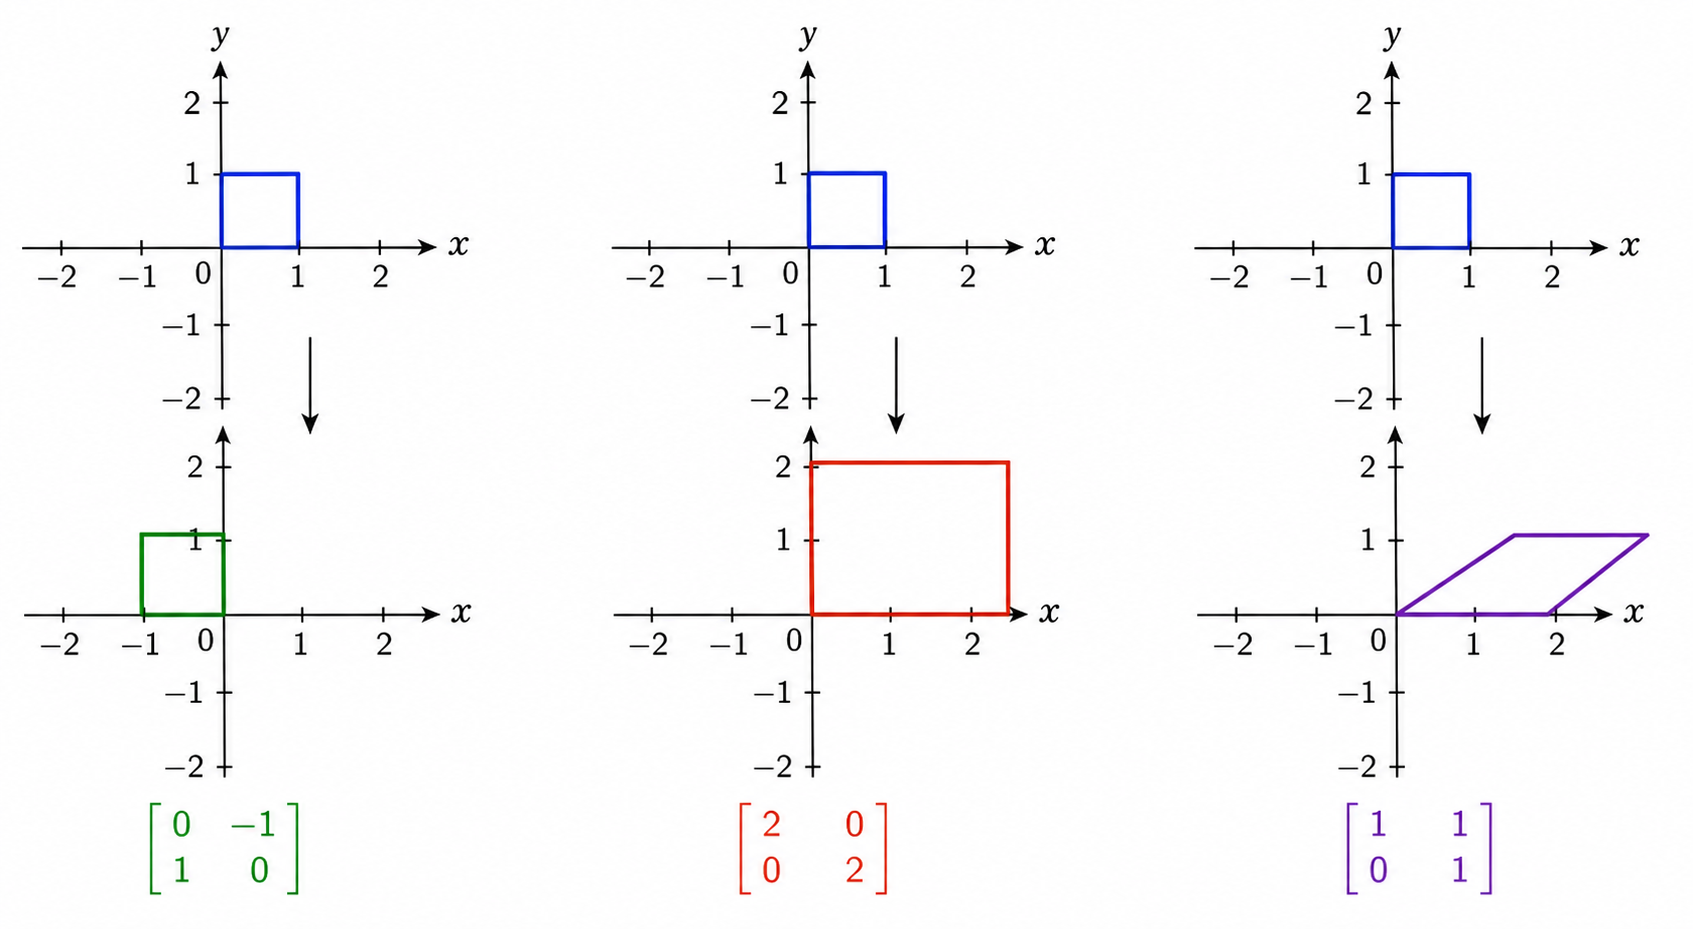
\includegraphics[width=0.62\textwidth]{Figures/png_ready/34-matrix-transformation-manual.png}
    \caption{แผนภาพแสดงการหมุน การขยาย และการเฉือนด้วยเมทริกซ์}
    \label{fig:matrix-transformation}
\end{figure}

เมทริกซ์ใช้ในการแปลงภาพกราฟิก 2 มิติ และ 3 มิติ อย่างมีประสิทธิภาพ โดยการแปลงหลักๆ ประกอบด้วยการเลื่อน (translation) การขยายหรือหด (scaling) และการหมุน (rotation) ซึ่งสามารถเขียนในรูปเมทริกซ์ได้โดยใช้ homogeneous coordinates ซึ่งเป็นเทคนิคที่เพิ่มมิติให้กับจุดเพื่อให้การแปลงทุกรูปแบบสามารถเขียนในรูปการคูณเมทริกซ์ได้อย่างเป็นหนึ่งเดียว หลักการนี้ถูกนำไปใช้ในโปรแกรมกราฟิกทุกประเภทตั้งแต่การวาดรูปง่ายๆ ไปจนถึงเกม 3 มิติขั้นสูง

\begin{ex}[การแปลง 2 มิติ]
การแปลงจุด $(x, y)$ ในระบบ 2 มิติ สามารถเขียนในรูปเมทริกซ์ได้ดังนี้

\[
\begin{pmatrix} x' \\ y' \\ 1 \end{pmatrix} = T \begin{pmatrix} x \\ y \\ 1 \end{pmatrix}
\]

โดยใช้ homogeneous coordinates
\end{ex}
\begin{solution}
\begin{align*}
\text{เลื่อน:}\quad T &= \begin{pmatrix} 1 & 0 & t_x \\ 0 & 1 & t_y \\ 0 & 0 & 1 \end{pmatrix}, &
\text{ขยาย:}\quad S &= \begin{pmatrix} s_x & 0 & 0 \\ 0 & s_y & 0 \\ 0 & 0 & 1 \end{pmatrix}\\
\text{หมุน:}\quad R &= \begin{pmatrix} \cos\theta & -\sin\theta & 0 \\ \sin\theta & \cos\theta & 0 \\ 0 & 0 & 1 \end{pmatrix}
\end{align*}
การแปลงผสม: $P' = T\cdot R\cdot S\cdot P$ \solhere
\end{solution}

\begin{ex}
หมุนจุด $(1, 0)$ รอบจุดกำเนิด $90^\circ$ โดยใช้เมทริกซ์การหมุน $R = \begin{pmatrix} 0 & -1 & 0 \\ 1 & 0 & 0 \\ 0 & 0 & 1 \end{pmatrix}$
\end{ex}
\begin{solution}
\[
P' = RP = \begin{pmatrix} 0 & -1 & 0 \\ 1 & 0 & 0 \\ 0 & 0 & 1 \end{pmatrix}\begin{pmatrix} 1 \\ 0 \\ 1 \end{pmatrix} = \begin{pmatrix} 0 \\ 1 \\ 1 \end{pmatrix}
\]
$\therefore$ จุดใหม่คือ $(0,1)$ \solhere
\end{solution}

\subsection{การเข้ารหัส Hill Cipher}
Hill Cipher เป็นระบบเข้ารหัสแบบบล็อกที่พัฒนาโดย Lester Hill ในปี ค.ศ. 1929 โดยใช้ความรู้เรื่องเมทริกซ์เป็นพื้นฐาน ข้อความธรรมดาถูกแปลงเป็นเวกเตอร์ตัวเลข แล้วคูณด้วยเมทริกซ์กุญแจ $K$ ผลลัพธ์คือข้อความเข้ารหัส ความแข็งแกร่งของ Hill Cipher อยู่ที่การกระจายตัวอักษรแต่ละตัวไปยังหลายตำแหน่งในข้อความเข้ารหัส ทำให้การวิเคราะห์ความถี่ตัวอักษร (frequency analysis) ไม่สามารถถอดรหัสได้โดยตรง

\begin{ex}
กำหนดเมทริกซ์กุญแจ $K = \begin{pmatrix} 3 & 2 \\ 1 & 1 \end{pmatrix}$ เข้ารหัสข้อความ ``HI''
\end{ex}
\begin{solution}
กำหนด A$=0$, \ldots, Z$=25$ จึงได้ H$=7$, I$=8$
\begin{align*}
P &= \begin{pmatrix} 7 \\ 8 \end{pmatrix}\\
C = KP &= \begin{pmatrix} 3 & 2 \\ 1 & 1 \end{pmatrix}\begin{pmatrix} 7 \\ 8 \end{pmatrix} = \begin{pmatrix} 37 \\ 15 \end{pmatrix} \equiv \begin{pmatrix} 11 \\ 15 \end{pmatrix} \pmod{26}
\end{align*}
$11=$L, $15=$P $\therefore$ ``HI'' $\to$ ``LP'' \solhere
\end{solution}

หมายเหตุ: การถอดรหัสต้องใช้ $K^{-1}$ ซึ่งมีอยู่ก็ต่อเมื่อ $\det(K) \neq 0 \pmod{26}$ นั่นคือ $\gcd(\det(K), 26) = 1$ ในกรณีนี้ $\det(K) = 3(1) - 2(1) = 1$ และ $\gcd(1, 26) = 1$ ดังนั้นตัวผกผันมีอยู่

\begin{ex}
ถอดรหัส ``LP'' กลับเป็น ``HI'' โดยใช้เมทริกซ์กุญแจ $K = \begin{pmatrix} 3 & 2 \\ 1 & 1 \end{pmatrix}$
\end{ex}
\begin{solution}
\begin{align*}
K^{-1} &= \begin{pmatrix} 1 & -2 \\ -1 & 3 \end{pmatrix} \pmod{26} \quad (\det K = 1)\\
P = K^{-1}C &= \begin{pmatrix} 1 & -2 \\ -1 & 3 \end{pmatrix}\begin{pmatrix} 11 \\ 15 \end{pmatrix} = \begin{pmatrix} -19 \\ 34 \end{pmatrix} \equiv \begin{pmatrix} 7 \\ 8 \end{pmatrix} \pmod{26}
\end{align*}
$7=$H, $8=$I $\therefore$ ได้ข้อความเดิม ``HI'' \solhere
\end{solution}

\subsection{เมทริกซ์ประชิดในทฤษฎีกราฟ}
เมทริกซ์ประชิดเป็นเครื่องมือสำคัญในการแทนกราฟในรูปแบบเมทริกซ์ ทำให้สามารถใช้คุณสมบัติทางพีชคณิตในการวิเคราะห์กราฟได้

\begin{ex}
Adjacency Matrix ของกราฟ $G$ ที่มี $n$ โหนด คือเมทริกซ์ $A$ ขนาด $n \times n$ โดยที่ $a_{ij} = 1$ ถ้ามีเส้นเชื่อมระหว่างโหนด $i$ และ $j$ และ $a_{ij} = 0$ ในกรณีอื่น โดยสมบัติที่สำคัญคือ $(A^k)_{ij}$ บอกจำนวนเส้นทางความยาว $k$ จากโหนด $i$ ไปยังโหนด $j$ และผลรวมของแถวที่ $i$ เท่ากับ degree ของโหนด $i$
\end{ex}
\begin{solution}
สร้าง $A_{n\times n}$ โดย $a_{ij}=1$ ถ้ามีเส้นเชื่อม $i$–$j$ มิฉะนั้น $0$; สมบัติ: $(A^k)_{ij}=$ จำนวนเส้นทางยาว $k$ จาก $i$ ไป $j$, และผลรวมแถว $i$ $=$ degree ของโหนด $i$ \solhere
\end{solution}

\begin{ex}
พิจารณากราฟรูปสามเหลี่ยม (3 โหนด เชื่อมกันทุกคู่) เมทริกซ์ประชิด (adjacency matrix) $A$ และกำลังสองของมันคือ
\[
A = \begin{pmatrix} 0 & 1 & 1 \\ 1 & 0 & 1 \\ 1 & 1 & 0 \end{pmatrix},
\qquad
A^2 = \begin{pmatrix} 2 & 1 & 1 \\ 1 & 2 & 1 \\ 1 & 1 & 2 \end{pmatrix}.
\]
สมาชิก $(A^2)_{ij}$ บอกจำนวนเส้นทาง 2 ขั้นจากโหนด $i$ ไปโหนด $j$ เช่น $(A^2)_{12} = 1$ หมายความว่ามี 1 เส้นทาง 2 ขั้นจากโหนด 1 ไปโหนด 2 (คือ $1 \to 3 \to 2$)
\end{ex}
\begin{solution}
\[
A = \begin{pmatrix} 0 & 1 & 1 \\ 1 & 0 & 1 \\ 1 & 1 & 0 \end{pmatrix} \Rightarrow A^2 = \begin{pmatrix} 2 & 1 & 1 \\ 1 & 2 & 1 \\ 1 & 1 & 2 \end{pmatrix}
\]
$(A^2)_{12}=1$: มี 1 เส้นทาง 2 ขั้น $1\to 3\to 2$; แนวทแยง $=2$ (แต่ละโหนดมี 2 เส้นทางกลับตัวเองผ่านโหนดอื่น) \solhere
\end{solution}

\subsection{เมทริกซ์ในการเรียนรู้ของเครื่อง}
ในการเรียนรู้ของเครื่อง (Machine Learning) ข้อมูลและพารามิเตอร์ของโมเดลมักถูกจัดเก็บในรูปเมทริกซ์ ทำให้การคำนวณจำนวนมหาศาลสรุปลงเหลือเพียงการคูณเมทริกซ์ไม่กี่ครั้ง ในที่นี้ยกตัวอย่างพื้นฐานสองแบบ คือ การถดถอยเชิงเส้น (Linear Regression) และโครงข่ายประสาทเทียม (Neural Network)

\begin{ex}[การถดถอยเชิงเส้น]
โมเดล Linear Regression เขียนในรูปเมทริกซ์เป็น $y = X\beta$ โดย $X$ คือเมทริกซ์ข้อมูล (design matrix) และ $\beta$ คือเวกเตอร์สัมประสิทธิ์ ค่าที่เหมาะที่สุดหาได้จาก normal equation $\beta = (X^T X)^{-1} X^T y$ จงหา $\beta$ สำหรับข้อมูล
\[
X = \begin{pmatrix} 1 & 2 \\ 1 & 4 \\ 1 & 6 \end{pmatrix}, \qquad
y = \begin{pmatrix} 3 \\ 5 \\ 7 \end{pmatrix}
\]
\end{ex}
\begin{solution}
\begin{align*}
X^T X &= \begin{pmatrix} 3 & 12 \\ 12 & 56 \end{pmatrix}, \quad \det = 24 \neq 0\\
(X^T X)^{-1} &= \tfrac{1}{24}\begin{pmatrix} 56 & -12 \\ -12 & 3 \end{pmatrix}, \quad X^T y = \begin{pmatrix} 15 \\ 68 \end{pmatrix}\\
\beta = (X^T X)^{-1} X^T y &= \begin{pmatrix} 1 \\ 1 \end{pmatrix}
\end{align*}
$\therefore y = 1 + x$ \solhere
\end{solution}

\begin{ex}[โครงข่ายประสาทเทียมหนึ่งชั้น]
โครงข่ายประสาทเทียมหนึ่งชั้น (single-layer neural network) คำนวณผลลัพธ์จาก $\mathbf{z} = \mathbf{x} W + \mathbf{b}$ แล้วส่งผ่านฟังก์ชันกระตุ้น (activation function) ReLU $f(z) = \max(0, z)$ จงหาผลลัพธ์ของชั้นนี้เมื่อ
\[
\mathbf{x} = \begin{pmatrix} 1 & 0.5 \end{pmatrix}, \qquad
W = \begin{pmatrix} 0.8 & 0.2 \\ 0.3 & 0.7 \end{pmatrix}, \qquad
\mathbf{b} = \begin{pmatrix} -0.5 & 0.1 \end{pmatrix}
\]
\end{ex}
\begin{solution}
\begin{align*}
\mathbf{z} &= \mathbf{x} W + \mathbf{b} = \begin{pmatrix} 1 & 0.5 \end{pmatrix}\begin{pmatrix} 0.8 & 0.2 \\ 0.3 & 0.7 \end{pmatrix} + \begin{pmatrix} -0.5 & 0.1 \end{pmatrix}\\
&= \begin{pmatrix} 0.95 & 0.55 \end{pmatrix} + \begin{pmatrix} -0.5 & 0.1 \end{pmatrix} = \begin{pmatrix} 0.45 & 0.65 \end{pmatrix}\\
f(\mathbf{z}) &= \mathrm{ReLU}(\mathbf{z}) = \begin{pmatrix} 0.45 & 0.65 \end{pmatrix}
\end{align*}
\solhere
\end{solution}

\sectionbanner{สรุปบทเรียน}
บทนี้ศึกษาเมทริกซ์และดีเทอร์มิแนนต์ซึ่งเป็นเครื่องมือพื้นฐานในคณิตศาสตร์และวิทยาการคอมพิวเตอร์ เริ่มจากเมทริกซ์ซึ่งเป็นการจัดเรียงข้อมูลในรูปตารางสองมิติและมีหลายประเภท เช่น เมทริกซ์จตุรัส เส้นทแยงมุม สมมาตร และสามเหลี่ยม ต่อด้วยการดำเนินการระหว่างเมทริกซ์ ได้แก่ การบวก ลบ คูณด้วยสเกลาร์ คูณเมทริกซ์ และการสลับเปลี่ยน (transpose) โดยการคูณเมทริกซ์ไม่มีสมบัติการสลับที่ ดีเทอร์มิแนนต์เป็นค่าจำเพาะของเมทริกซ์จตุรัสที่คำนวณได้ด้วยการกระจายโคแฟกเตอร์ (cofactor expansion) หรือกฎของ Sarrus สำหรับเมทริกซ์ $3 \times 3$ และมีสมบัติสำคัญคือ $\det(AB) = \det(A)\det(B)$ ตัวผกผัน $A^{-1}$ ทำให้ $AA^{-1} = A^{-1}A = I$ และมีได้ก็ต่อเมื่อ $\det(A) \neq 0$ ระบบสมการเชิงเส้นแก้ได้ด้วยตัวผกผันเมทริกซ์ ($x = A^{-1}b$) กฎของคราเมอร์ หรือการกำจัดแบบเกาส์ (Gaussian elimination) และนำไปประยุกต์ในคอมพิวเตอร์กราฟิกส์ การเข้ารหัส การเรียนรู้ของเครื่อง และทฤษฎีกราฟ

เมทริกซ์เป็นพื้นฐานที่จำเป็นสำหรับการศึกษาต่อในสาขาคณิตศาสตร์ขั้นสูง เช่น พีชคณิตเชิงเส้น (Linear Algebra) และการวิเคราะห์เชิงตัวเลข (Numerical Analysis)~\cite{strang2023linear}

\clearpage
\sectionbanner{แบบฝึกหัด}
\exercisepart{ส่วนที่ 1: พื้นฐานเมทริกซ์}
\begin{exercise}
จงระบุขนาดของเมทริกซ์ต่อไปนี้
\begin{enumerate}
    \item $A = \begin{pmatrix} 1 & 2 & 3 \\ 4 & 5 & 6 \end{pmatrix}$
    \item $B = \begin{pmatrix} 1 & 0 \\ 0 & 1 \\ 1 & 0 \end{pmatrix}$
    \item $C = \begin{pmatrix} 3 \end{pmatrix}$
\end{enumerate}
\end{exercise}

\begin{exercise}
จงระบุว่าเมทริกซ์ต่อไปนี้เป็นเมทริกซ์ชนิดใด (จตุรัส, สมมาตร, สามเหลี่ยมบน, สามเหลี่ยมล่าง, เส้นทแยงมุม, เอกลักษณ์, ศูนย์)
\begin{enumerate}
    \item $A = \begin{pmatrix} 1 & 0 & 0 \\ 0 & 2 & 0 \\ 0 & 0 & 3 \end{pmatrix}$
    \item $B = \begin{pmatrix} 1 & 2 \\ 2 & 1 \end{pmatrix}$
    \item $C = \begin{pmatrix} 1 & 1 & 1 \\ 0 & 1 & 1 \\ 0 & 0 & 1 \end{pmatrix}$
\end{enumerate}
\end{exercise}

\exercisepart{ส่วนที่ 2: การดำเนินการระหว่างเมทริกซ์}
\begin{exercise}
กำหนด $A = \begin{pmatrix} 1 & 2 \\ 3 & 4 \end{pmatrix}$ และ $B = \begin{pmatrix} 5 & 6 \\ 7 & 8 \end{pmatrix}$ จงหา
\begin{enumerate}
    \item $A + B$
    \item $A - B$
    \item $3A$
    \item $A \cdot B$
    \item $B \cdot A$
\end{enumerate}
\end{exercise}

\begin{exercise}
จงหา transpose ของเมทริกซ์ต่อไปนี้
\begin{enumerate}
    \item $A = \begin{pmatrix} 1 & 2 & 3 \\ 4 & 5 & 6 \end{pmatrix}$
    \item $B = \begin{pmatrix} 1 & 2 \\ 3 & 4 \\ 5 & 6 \end{pmatrix}$
\end{enumerate}
\end{exercise}

\exercisepart{ส่วนที่ 3: ดีเทอร์มิแนนต์}
\begin{exercise}
จงคำนวณดีเทอร์มิแนนต์ของเมทริกซ์ต่อไปนี้โดยใช้วิธี cofactor expansion:
\begin{enumerate}
    \item $\det\begin{pmatrix} 1 & 2 \\ 3 & 4 \end{pmatrix}$
    \item $\det\begin{pmatrix} 1 & 0 & 2 \\ 3 & 1 & 4 \\ 5 & 6 & 1 \end{pmatrix}$
\end{enumerate}
\end{exercise}

\begin{exercise}
จงคำนวณดีเทอร์มิแนนต์โดยใช้กฎของ Sarrus:
\begin{enumerate}
    \item $\det\begin{pmatrix} 1 & 2 & 3 \\ 4 & 5 & 6 \\ 7 & 8 & 9 \end{pmatrix}$
\end{enumerate}
\end{exercise}

\exercisepart{ส่วนที่ 4: ตัวผกผันของเมทริกซ์}
\begin{exercise}
จงหาตัวผกผันของเมทริกซ์ต่อไปนี้ (ถ้ามี)
\begin{enumerate}
    \item $A = \begin{pmatrix} 1 & 2 \\ 3 & 4 \end{pmatrix}$
    \item $B = \begin{pmatrix} 2 & 1 \\ 4 & 2 \end{pmatrix}$
    \item $I = \begin{pmatrix} 1 & 0 & 0 \\ 0 & 1 & 0 \\ 0 & 0 & 1 \end{pmatrix}$
\end{enumerate}
\end{exercise}

\begin{exercise}
จงตรวจสอบว่า $A \cdot A^{-1} = A^{-1} \cdot A = I$ สำหรับข้อ 1(a)
\end{exercise}

\exercisepart{ส่วนที่ 5: การแก้ระบบสมการเชิงเส้น}
\begin{exercise}
จงแก้ระบบสมการต่อไปนี้โดยใช้ตัวผกผันเมทริกซ์
\begin{enumerate}
    \item $x + 2y = 5,\ 3x + 4y = 6$
    \item $2x + y = 3,\ x - y = 1$
\end{enumerate}
\end{exercise}

\begin{exercise}
จงแก้ระบบสมการต่อไปนี้โดยใช้กฎของคราเมอร์
\begin{enumerate}
    \item $x + y = 2,\ 2x + 3y = 5$
\end{enumerate}
\end{exercise}

\clearpage
\answerkeyhead
เฉลยอย่างย่อสำหรับแบบฝึกหัดในแต่ละส่วน เพื่อให้ผู้เรียนใช้ตรวจคำตอบของตนเอง

\exercisepart{ส่วนที่ 1: พื้นฐานเมทริกซ์}
\begin{enumerate}[label={},leftmargin=0pt]
    \item ขนาด
    \begin{enumerate}[label=\textbf{\thechapter.\arabic{enumi}.\arabic*}]
        \item $2\times 3$
        \item $3\times 2$
        \item $1\times 1$
    \end{enumerate}

    \item ประเภท
    \begin{enumerate}[label=\textbf{\thechapter.\arabic{enumi}.\arabic*}]
        \item จตุรัส เส้นทแยงมุม (และเป็นสมมาตร สามเหลี่ยมบน สามเหลี่ยมล่างพร้อมกัน)
        \item จตุรัส สมมาตร
        \item จตุรัส สามเหลี่ยมบน
    \end{enumerate}
\end{enumerate}

\exercisepart{ส่วนที่ 2: การดำเนินการระหว่างเมทริกซ์}
\begin{enumerate}[label={},leftmargin=0pt,start=3]
    \item การดำเนินการ
    \begin{enumerate}[label=\textbf{\thechapter.\arabic{enumi}.\arabic*}]
        \item $A+B = \begin{pmatrix}6 & 8\\ 10 & 12\end{pmatrix}$
        \item $A-B = \begin{pmatrix}-4 & -4\\ -4 & -4\end{pmatrix}$
        \item $3A = \begin{pmatrix}3 & 6\\ 9 & 12\end{pmatrix}$
        \item $AB = \begin{pmatrix}19 & 22\\ 43 & 50\end{pmatrix}$
        \item $BA = \begin{pmatrix}23 & 34\\ 31 & 46\end{pmatrix}$ (ยืนยันว่า $AB\neq BA$)
    \end{enumerate}

    \item เมทริกซ์สลับเปลี่ยน
    \begin{enumerate}[label=\textbf{\thechapter.\arabic{enumi}.\arabic*}]
        \item $A^T = \begin{pmatrix}1 & 4\\ 2 & 5\\ 3 & 6\end{pmatrix}$
        \item $B^T = \begin{pmatrix}1 & 3 & 5\\ 2 & 4 & 6\end{pmatrix}$
    \end{enumerate}
\end{enumerate}

\exercisepart{ส่วนที่ 3: ดีเทอร์มิแนนต์}
\begin{enumerate}[label={},leftmargin=0pt,start=5]
    \item ดีเทอร์มิแนนต์
    \begin{enumerate}[label=\textbf{\thechapter.\arabic{enumi}.\arabic*}]
        \item $\det = (1)(4)-(2)(3) = -2$
        \item กระจายตามแถวที่ 1: $1\cdot(1-24) - 0 + 2\cdot(18-5) = -23 + 26 = 3$
    \end{enumerate}
    \item Sarrus: $aei+bfg+cdh-ceg-bdi-afh = 45+84+96-105-72-48 = 0$
\end{enumerate}

\exercisepart{ส่วนที่ 4: ตัวผกผันของเมทริกซ์}
\begin{enumerate}[label={},leftmargin=0pt,start=7]
    \item การหาตัวผกผัน
    \begin{enumerate}[label=\textbf{\thechapter.\arabic{enumi}.\arabic*}]
        \item $\det(A) = -2 \neq 0$, $A^{-1} = -\frac{1}{2}\begin{pmatrix}4 & -2\\ -3 & 1\end{pmatrix} = \begin{pmatrix}-2 & 1\\ \frac{3}{2} & -\frac{1}{2}\end{pmatrix}$
        \item $\det(B) = 0$ จึงไม่มีตัวผกผัน
        \item $I^{-1} = I$
    \end{enumerate}
    \item $A\cdot A^{-1} = \begin{pmatrix}1 & 2\\ 3 & 4\end{pmatrix}\begin{pmatrix}-2 & 1\\ \frac{3}{2} & -\frac{1}{2}\end{pmatrix} = \begin{pmatrix}1 & 0\\ 0 & 1\end{pmatrix} = I$ และตรวจ $A^{-1}\cdot A = I$ เช่นกัน
\end{enumerate}

\exercisepart{ส่วนที่ 5: การแก้ระบบสมการเชิงเส้น}
\begin{enumerate}[label={},leftmargin=0pt,start=9]
    \item การแก้ระบบสมการด้วยตัวผกผัน
    \begin{enumerate}[label=\textbf{\thechapter.\arabic{enumi}.\arabic*}]
        \item $A^{-1}b = \begin{pmatrix}-2 & 1\\ \frac{3}{2} & -\frac{1}{2}\end{pmatrix}\begin{pmatrix}5\\ 6\end{pmatrix} = \begin{pmatrix}-4\\ \frac{9}{2}\end{pmatrix}$ ดังนั้น $x=-4, y=\frac{9}{2}$
        \item $\det(A) = -3$, $A^{-1} = -\frac{1}{3}\begin{pmatrix}-1 & -1\\ -1 & 2\end{pmatrix} = \begin{pmatrix}\frac{1}{3} & \frac{1}{3}\\ \frac{1}{3} & -\frac{2}{3}\end{pmatrix}$ ดังนั้น $\begin{pmatrix}x\\y\end{pmatrix} = A^{-1}b = \begin{pmatrix}\frac{1}{3} & \frac{1}{3}\\ \frac{1}{3} & -\frac{2}{3}\end{pmatrix}\begin{pmatrix}3\\1\end{pmatrix} = \begin{pmatrix}\frac{4}{3}\\ \frac{1}{3}\end{pmatrix}$
    \end{enumerate}
    \item กฎคราเมอร์ $\det A = 1$, $\det A_x = \begin{vmatrix}2 & 1\\ 5 & 3\end{vmatrix} = 1$, $\det A_y = \begin{vmatrix}1 & 2\\ 2 & 5\end{vmatrix} = 1$ ดังนั้น $x = 1, y = 1$
\end{enumerate}

\newpage
\QAChapter
\begin{enumerate}
    \item จงระบุขนาดของเมทริกซ์ต่อไปนี้ และระบุจำนวนสมาชิกทั้งหมด
    \begin{enumerate}
        \item $A = \begin{pmatrix} 1 & 2 & 3 \\ 4 & 5 & 6 \end{pmatrix}$
        \item $B = \begin{pmatrix} 1 & 0 \\ 0 & 1 \\ 1 & 0 \end{pmatrix}$
        \item $C = \begin{pmatrix} 3 \end{pmatrix}$
    \end{enumerate}
    \item จงบอกประเภทของเมทริกซ์ต่อไปนี้ (จตุรัส, สมมาตร, สามเหลี่ยมบน, สามเหลี่ยมล่าง, เส้นทแยงมุม, เอกลักษณ์, ศูนย์)
    \begin{enumerate}
        \item $A = \begin{pmatrix} 1 & 0 & 0 \\ 0 & 2 & 0 \\ 0 & 0 & 3 \end{pmatrix}$
        \item $B = \begin{pmatrix} 1 & 2 \\ 2 & 1 \end{pmatrix}$
        \item $C = \begin{pmatrix} 1 & 1 & 1 \\ 0 & 1 & 1 \\ 0 & 0 & 1 \end{pmatrix}$
    \end{enumerate}
    \item กำหนด $A = \begin{pmatrix} 1 & 2 \\ 3 & 4 \end{pmatrix}$ และ $B = \begin{pmatrix} 5 & 6 \\ 7 & 8 \end{pmatrix}$ จงหา $A + B$, $A - B$, $3A$, $A \cdot B$, และ $B \cdot A$
    \item จงพิสูจน์ว่า $(AB)^T = B^T A^T$ สำหรับเมทริกซ์ $A$ และ $B$ ขนาด $2 \times 2$
    \item จงคำนวณดีเทอร์มิแนนต์ของเมทริกซ์ต่อไปนี้โดยวิธี cofactor expansion:
    \begin{enumerate}
        \item $\det\begin{pmatrix} 1 & 2 \\ 3 & 4 \end{pmatrix}$
        \item $\det\begin{pmatrix} 1 & 0 & 2 \\ 3 & 1 & 4 \\ 5 & 6 & 1 \end{pmatrix}$
    \end{enumerate}
    \item จงหาตัวผกผันของ $A = \begin{pmatrix} 2 & 1 \\ 1 & 1 \end{pmatrix}$ (ถ้ามี) และตรวจสอบ $A \cdot A^{-1} = I$
    \item จงแก้ระบบสมการ $x + 2y = 5,\ 3x + 4y = 11$ โดยใช้ตัวผกผันเมทริกซ์
    \item จงอธิบายการประยุกต์ใช้เมทริกซ์ในงานด้านคอมพิวเตอร์กราฟิกส์ พร้อมยกตัวอย่างการแปลงเมทริกซ์
\end{enumerate}

\newpage
\sheetChapter{เมทริกซ์และดีเทอร์มิแนนต์ (Matrices \& Determinants)}
\section*{วัตถุประสงค์}
\begin{enumerate}
    \item เพื่อให้ผู้เรียนเข้าใจนิยามและประเภทของเมทริกซ์
    \item เพื่อให้ผู้เรียนสามารถดำเนินการบวก ลบ คูณเมทริกซ์ได้
    \item เพื่อให้ผู้เรียนคำนวณดีเทอร์มิแนนต์และหาตัวผกผันได้
    \item เพื่อให้ผู้เรียนประยุกต์ใช้เมทริกซ์ในการแก้ระบบสมการเชิงเส้น
\end{enumerate}
\section*{คำชี้แจง} ให้ผู้เรียนศึกษาเนื้อหาบทเมทริกซ์และดีเทอร์มิแนนต์ แล้วตอบคำถามต่อไปนี้
\begin{enumerate}
    \item ให้ผู้เรียนอธิบายความหมายของเมทริกซ์ พร้อมยกตัวอย่างเมทริกซ์ขนาด $3 \times 2$
    \Pointilles{3}
    \item ให้ผู้เรียนยกตัวอย่างเมทริกซ์ประเภทต่างๆ ที่กล่าวในบทเรียน
    \Pointilles{3}
    \item ให้ผู้เรียนอธิบายขั้นตอนการคูณเมทริกซ์ $A_{m \times n} \cdot B_{n \times p}$ พร้อมยกตัวอย่าง
    \Pointilles{3}
    \item ให้ผู้เรียนสรุปสมบัติของดีเทอร์มิแนนต์ที่สำคัญ
    \Pointilles{3}
    \item ให้ผู้เรียนอธิบายเงื่อนไขที่เมทริกซ์จะมีตัวผกผัน พร้อมยกตัวอย่าง
    \Pointilles{3}
    \item ให้ผู้เรียนอธิบายการประยุกต์ใช้เมทริกซ์ในงานด้านวิทยาการคอมพิวเตอร์อย่างน้อย 2 ตัวอย่าง
    \Pointilles{3}
\end{enumerate}
